\documentclass[main.tex]{subfiles}
\begin{document}

\href{https://www2.seas.gwu.edu/~simhaweb/quantum/modules/module2/module2.html}{Module 2 Quantum Linear Algebra Part I}

\subsection{Why do we need the linear algebra of complex vectors?}

    We will over the course develop intuition for why we need complex-number vectors and certain types of matrices.And we will see mathematical reasons for why complex vectors emerge from simple observations and basic assumptions. For now, we'll provide a high-level operational view as motivation. Let's start by recalling how a standard electronic circuit (in a calculator or computer) performs an arithmetic operation as shown in Figure \ref{fig:01addition}. Here, a binary number sits in a device (called a register) that holds bits (the number's digits). These bits then flow into a logic circuit, which we've seen earlier consists of a collection of Boolean gates (like AND, OR and NOT gates). The gates together achieve the desired computation (increment, in the above example), and the resulting number is fed back into the register. This conceptual description is reasonably close to what happens physically inside a calculator or computer.

    \begin{figure}
        \centering
        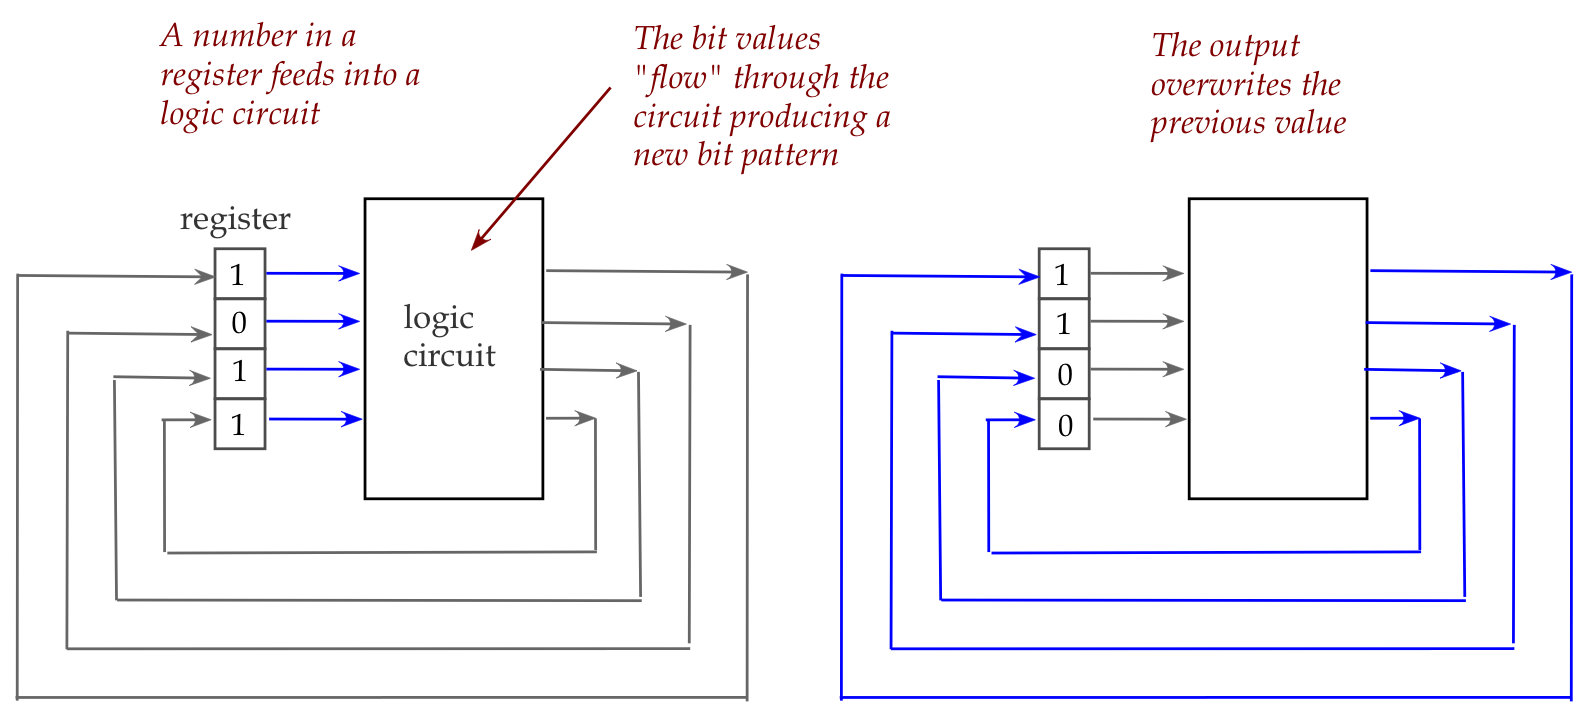
\includegraphics[width=4in]{notes/figs/n04/01circuit.png}
        \caption{Binary Register and Logical Circuit}
        \label{fig:01addition}
    \end{figure}
    
    The quantum equivalent is shown in Figure \ref{fig:02circuit2}. For the moment we will describe a conceptual view that is actually implemented in wildly different ways. The actual physical implementation can be quite different. The starting point is not a binary number but a (complex) vector. We will see that each qubit is actually a small vector. A collection of qubits is also a (larger) vector. Just as logic gates "act" on regular bits, in a quantum circuit it is matrices that "act" on vectors. There are going to be two fundamentally different kinds of matrices, and they "act" quite differently. One kind is called unitary and acts in the way we're already familiar with: the matrix multiplies into the input vector. The other kind is called Hermitian and the way it "acts" on a vector is a little strange. In a physical realization, of course, there are physical devices (such as lasers) that achieve the job of these matrices. Thus, there's no getting around the need to be really comfortable with the essential linear algebra needed for quantum computing: the linear algebra of complex vectors with two special types of matrices.
    
    \begin{figure}
        \centering
        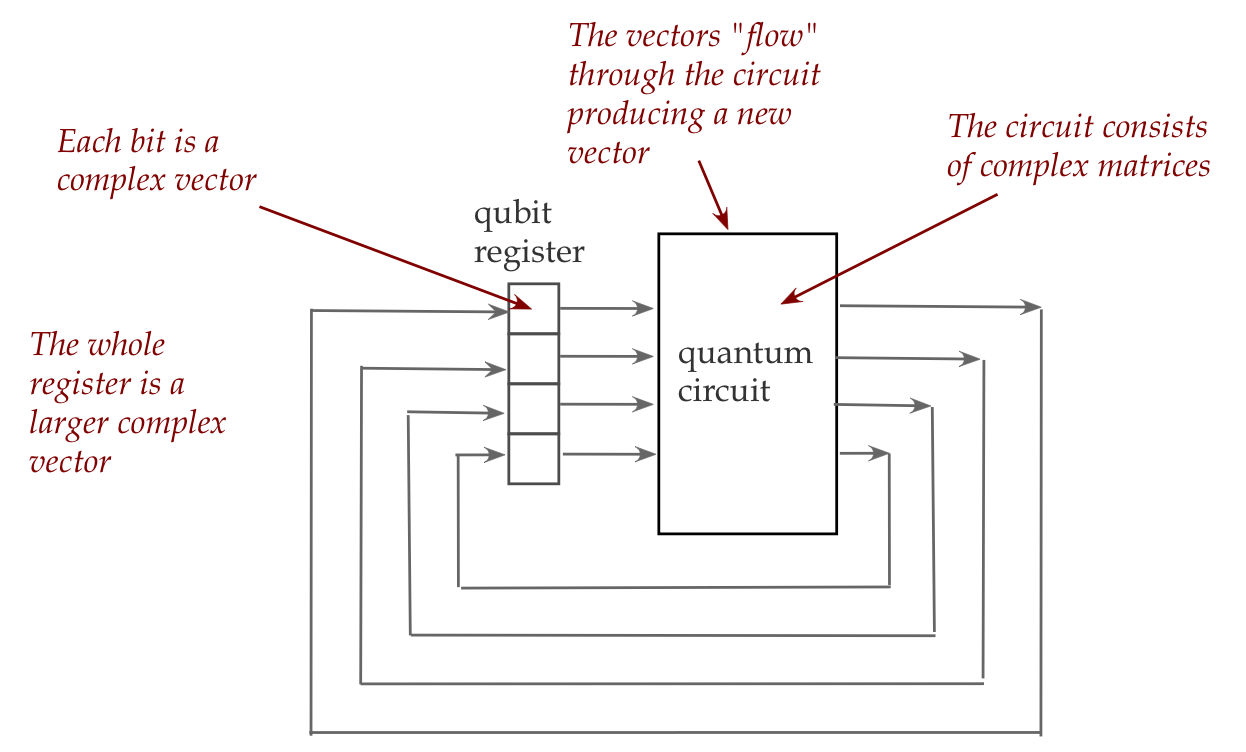
\includegraphics[width=4in]{notes/figs/n04/02circuit2.png}
        \caption{Qubit Register and Quantum Circuit}
        \label{fig:02circuit2}
    \end{figure}

\subsection{Complex numbers: a review}

    What are they and where did they come from? Consider an equation like $x^{2}=4$. We know that $x=2$ and $x=-2$ are solutions (written as $x=\pm 2$ ). What about $x^{2}=2$? Doesn't change the concept: $x=\pm \sqrt{2}$. However, $x^{2}=-2$ poses a problem. No square of a real number is negative Suppose we invent the "number" $\sqrt{-1}$ and give it a symbol:
    
    $$i=\sqrt{-1}$$
    
    Then using the rules of algebra
    
    $$(i \sqrt{2})^{2}=i^{2}(\sqrt{2})^{2}=(\sqrt{-1})^{2}(\sqrt{2})^{2}=(-1)(2)=-2$$
    
    gives a solution to the previous equation. In general, a complex number is written as $a+i b$ where $a$ and $b$ are real numbers. The $a$ in $a+i b$ is called the real part. $b$ is called the imaginary part. Why should this make sense? We want to include all real numbers in the set of complex numbers This works when $b=0$ in $a+i b$. However, we need to define arithmetic operations carefully so that when $b=0$ the same operations work for real numbers. That is, operations defined on complex numbers should give the expected results when applied to complex numbers with only real parts Luckily, the straightforward algebra works.
    * Addition: $(a+i b)+(c+i d) \triangleq(a+c)+i(b+d)$
    * Multiplication: $(a+i b)(c+i d) \triangleq(a c-b d)+i(a d+b c)$
    Notice: we simply treated the real numbers $a, b, c, d$ and $i$ as symbols and used standard algebra (factoring and distribution). Notice that the addition rule satisfies our original starting point with $a=0, b=1$ :
    
    $$(0+i)(0+i)=\left(00+0 i+0 i+i^{2}\right)=i^{2}=-1$$
    
    Multiplication by a real-number scalar:
    
    $$\beta(a+i b)=(\beta a+i(\beta b))$$
    
    Subtraction and division: Subtraction simply negates the real numbers of the second complex number, as in:
    
    $$(a+i b)-(c+i d)=(a+i b)+((-c)+i(-d))$$
    
    Division needs a bit more thought:
    
    $$\frac{a+i b}{c+i d}=\frac{a+i b}{c+i d} \frac{c-i d}{c-i d}=\frac{1}{c^{2}+d^{2}}(a+i b)(c-i d)$$

    Which now becomes a multiplication of two complex numbers, followed by a scalar multiplication. Note: we exploited the cancellation in
    
    $$(c+i d)(c-i d)=c^{2}-i^{2} d^{2}+(c)(i d)-(c)(i d)=c^{2}+d^{2}$$ 

    Notation: We will typically write a complex number symbolically as $a+i b$. But particular values might be written as $3+4 i$ because that's more natural than $3+i 4$. It takes some getting used to, but you should see $3+4 i$ as one number. When reading, your eyes should locate the $i$ in $3+4 i$ so that you separately see the imaginary part 4.\\
    
    About the meaning of a complex number: A real number always has physical interpretations, like length. A complex does not directly correspond to anything physical. Instead, it's best to think of it as abstraction that leads to predictive power. When we need to predict a physical quantity, we'll be sure to extract a real number.\\
    
    We should also point out a downside to complex numbers: there's no natural ordering. We can't say whether $3+4 i$ is less than $4+3 i$ or the other way around. Fortunately, this issue is not going to impact our needs.\\

    For Polar representation of complex numbers, one useful graphical representation shown in Figure \ref{03complexnumber} is obvious when we write complex number $z$ as $z=x+i y$.\\
    
    \begin{figure}
        \centering
        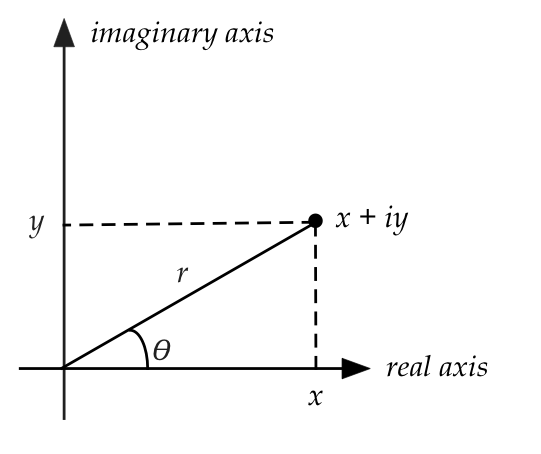
\includegraphics[width=3in]{notes/figs/n04/03complexnumber.png}
        \caption{Complex Number real and imaginary axis}
        \label{fig:03complexnumber}
    \end{figure}
    
    Given this, one can easily write
    
    \begin{align*}
    z   &=x+i y \\
        &=r \cos (\theta)+i r \sin (\theta) \\
        &=r(\cos (\theta)+i \sin (\theta))
    \end{align*}
    
    Once arithmetic has been defined, we can define functions on complex numbers: An important observation made by Euler: Suppose you define
    
    $$e^{z} \triangleq 1+z+\frac{z^{2}}{2 !}+\frac{z^{3}}{3 !}+\ldots$$
    
    analogous to the Taylor series for the real function $e^{x}$
    
    $$e^{x}=1+x+\frac{x^{2}}{2 !}+\frac{x^{3}}{3 !}+\ldots$$
    
    Then substituting $z=i \theta$, and separating out alternate terms:
    
    \begin{align*}
    e^{i \theta}    &=1+i \theta+\frac{(i \theta)^{2}}{2 !}+\frac{(i \theta)^{3}}{3 !}+\ldots \\
                    &=(\operatorname{series} \text { for } \cos (\theta))+i(\text { series for } \sin (\theta)) \\
                    &=\cos (\theta)+i \sin (\theta)
    \end{align*}
    
    This is called Euler's relation. More generally, $r e^{i \theta}=r(\cos (\theta)+i \sin (\theta))$ Think of $z=r e^{i \theta}$ as the polar representation of the complex number
    
    $$z=x+i y=r(\cos (\theta)+i \sin (\theta))$$
    
    Let's revisit some operations with the polar form $z_{1}=r_{1} e^{i \theta_{1}}$ and $z_{2}=r_{2} e^{i \theta_{2}}$
    
    \begin{align*}
    z_{1} z_{2} &=r_{1} r_{2} e^{i\left(\theta_{1}+\theta_{2}\right)} \\
    \frac{z_{1}}{z_{2}} &=\frac{r_{1}}{r_{2}} e^{i\left(\theta_{1}-\theta_{2}\right)} \\
    z_{1}^{-1} &=\frac{1}{r_{1}} e^{-i \theta_{1}}
    \end{align*}
    
    Sometimes an abundance of parentheses can be confusing, so we often $\operatorname{simplify} r(\cos (\theta)+i \sin (\theta))$ to
    
    $$r(\cos \theta+i \sin \theta).$$
    
    where it's understood that $\theta$ is the argument to $\cos$ and $\sin$. Redundancy in $\theta$ : While different values of $a$ and $b$ will result in different complex numbers $a+i b$, the same is not true for $r, \theta$. Because, for any integer $k$
    
    \begin{align*}
    \sin (\theta+2 \pi k) &=\sin \theta \\
    \cos (\theta+2 \pi k) &=\cos \theta
    \end{align*}
    
    In polar form
    
    $$e^{i(\theta+2 \pi k)}=e^{i \theta}$$
    
    Thus, for example, $3 e^{i\left(\frac{\pi}{3}+6 \pi\right)}$ and $3 e^{i \frac{\pi}{3}}$ are the same number. Thus, two numbers in polar form $r_{1} e^{i \theta_{1}}$ and $r_{2} e^{i \theta_{2}}$ are equal if and only if $r_{1}=r_{2}$ and $\theta_{1}=\theta_{2}+2 \pi k$ for some integer $k$.\\
    
    Conjugates: It turns out to be really useful to define something called a conjugate of a complex number $z=a+i b$:
    
    \begin{align*}
    z^{*} &=(a+i b)^{*} \\
    & \triangleq a-i b
    \end{align*}
    
    Then,
    
    \begin{align*}
    z z^{*} &=(a+i b)(a+i b)^{*} \\
    &=(a+i b)(a-i b) \\
    &=a^{2}+b^{2}
    \end{align*}
    
    Which is a real number. The magnitude of a complex number $z=a+i b$ is the real number
    
    $$|z| \triangleq \sqrt{a^{2}+b^{2}}=\sqrt{z z^{*}}=\sqrt{z^{*} z}$$
    
    The magnitude, we have seen, has a geometrical interpretation to complex numbers: the distance from the origin to the point representing $z$ as seen in Figure \ref{fig:04complexnumber2}.
    
    \begin{figure}
        \centering
        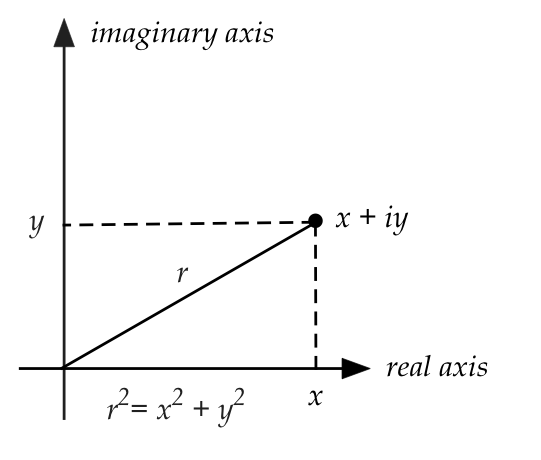
\includegraphics[width=3in]{notes/figs/n04/04complexnumber2.png}
        \caption{Complex Number Magnitude}
        \label{fig:04complexnumber2}
    \end{figure}
    
    Thus, in polar form
    
    $$\left|r e^{i \theta}\right|=|r|\left|e^{i \theta}\right|=r$$
    
    because $\left|e^{i \theta}\right|^{2}=|\cos \theta+i \sin \theta|^{2}=\cos ^{2} \theta+\sin ^{2} \theta=1$. Useful rules to remember about conjugation:
    
    \begin{align*}
    \left(z^{*}\right)^{*} &=z \\
    \left(z_{1}+z_{2}\right)^{*} &=z_{1}^{*}+z_{2}^{*} \\
    \left(z_{1}-z_{2}\right)^{*} &=z_{1}^{*}-z_{2}^{*} \\
    \left(z_{1} z_{2}\right)^{*} &=z_{1}^{*} z_{2}^{*} \\
    \left(\frac{z_{1}}{z_{2}}\right)^{*} &=\frac{z_{1}^{*}}{z_{2}^{*}}
    \end{align*}
    
    And, most importantly, the polar form of conjugation:
    
    $$
    \begin{aligned}
    \left(r e^{i \theta}\right)^{*} &=(r(\cos \theta+i \sin \theta))^{*} \\
    &=r(\cos \theta-i \sin \theta) \\
    &=r(\cos \theta+i \sin (-\theta)) \\
    &=r e^{-i \theta}
    \end{aligned}
    $$
    
    Note: we used parens only when needed above. We will commonly see the case when $r=1$ (unit length), in which case it simplifies to $e^{-i \theta}$. Alternate notation for conjugation: Math books often use a "bar" to denote conjugation:
    
    $$
    \begin{aligned}
    \bar{z} &=\overline{a+i b} \\
    &=a-i b
    \end{aligned}
    $$
    
    We will generally prefer the * notation because we'll want to conjugate entire matrices. Additional notation: Notation for the real and imaginary parts of $z=a+i b$ :
    
    $$
    \begin{aligned}
    &\operatorname{Re} z=a \\
    &\operatorname{Im} z=b
    \end{aligned}
    $$
    
    To extract the polar angle, one uses arg, but because many angles are equivalent, one gets a set:
    
    $$
    \arg z=\left\{\theta: r e^{i \theta}=z\right\}
    $$
    
    When a particular angle is specified, as in $2 e^{i \frac{\pi}{3}}$, then the angle (in radians) is often called the phase. Notice that multiplication by $e^{i \phi}$ changes the phase:
    
    $$
    e^{i \phi} 2 e^{i \frac{\pi}{3}}=2 e^{i\left(\frac{\pi}{3}+\phi\right)}
    $$
    
    This is a notion we will return to frequently in the future.

\subsection{Complex vectors (in old notation)}

    Because the Dirac notation takes getting used to, we'll first look at complex vectors in the notation used in linear algebra courses. A vector with complex numbers as elements is a complex vector: Thus, if $2+3 i$ and $5-4 i$ are two complex numbers, the vector $(2+3 i, 5-4 i)$ is a $2 \mathrm{D}$ complex vector. But because the complex numbers include reals, $(1.5,2)$ is also a complex vector. In general, a complex vector of $n$ dimensions will have $n$ complex numbers as elements:
    
    $$
    \left(a_{1}+i b_{1}, a_{2}+i b_{2}, \ldots, a_{n}+i b_{n}\right)
    $$
    
    In column form:
    
    $$
    \left[\begin{array}{r}
    a_{1}+i b_{1} \\
    a_{2}+i b_{2} \\
    \vdots \\
    a_{n}+i b_{n}
    \end{array}\right]
    $$
    
    What remains is to see how the operations on real vectors can be extended to complex vectors. Addition is a straightforward extension: Let $\mathbf{u}=\left(u_{1}, \ldots, u_{n}\right)$ and $\mathbf{v}=\left(v_{1}, \ldots, v_{n}\right)$ be two complex vectors. Here, each $u_{i}$ and $v_{j}$ are complex numbers, with real and imaginary parts. Then,
    
    $$
    \mathbf{u}+\mathbf{v}=\left(u_{1}+v_{1}, u_{2}+v_{2}, \ldots, u_{n}+v_{n}\right)
    $$
    
    Each $u_{i}+v_{i}$ is complex addition. Example:
    
    $$
    \left[\begin{array}{r}
    1+2 i \\
    i \\
    -3+4 i
    \end{array}\right]+\left[\begin{array}{r}
    -2+i \\
    2 \\
    4
    \end{array}\right]=\left[\begin{array}{r}
    -1+3 i \\
    2+i \\
    1+4 i
    \end{array}\right]
    $$
    
    Scalar multiplication is a bit different in that the scalar can now be a complex number:
    
    $$
    \begin{aligned}
    \alpha \mathbf{u} &=\alpha\left(u_{1}, u_{2}, \ldots, u_{n}\right) \\
    &=\left(\alpha u_{1}, \alpha u_{2}, \ldots, \alpha u_{n}\right)
    \end{aligned}
    $$
    
    Here, both $\alpha$ and each $u_{i}$ are complex numbers. Thus, the rules of complex multiplication are needed for calculating each $\alpha u_{i}$. Example:
    
    $$
    (1-2 i)\left[\begin{array}{r}
    1+2 i \\
    3
    \end{array}\right]=\left[\begin{array}{r}
    5 \\
    3-6 i
    \end{array}\right]
    $$
    
    So far, operations for complex vectors look like their real counterparts. The dot product, however, is an exception. For complex vectors $\mathbf{u}$ and $\mathbf{v}$, the dot (inner) product is defined as
    
    $$
    \mathbf{u} \cdot \mathbf{v}=u_{1}^{*} v_{1}+u_{2}^{*} v_{2}+\ldots+u_{n}^{*} v_{n}
    $$
    
    Recall: for a complex number $z=a+b i, z^{*}=\operatorname{conjugate}(z)=a-b i$. Example: $\mathbf{u}=(1,2-i, 3 i), \mathbf{v}=(2,1, i)$
    
    $$
    \begin{aligned}
    \mathbf{u} \cdot \mathbf{v} &=(1,2-i, 3 i)^{*} \cdot(2,1, i) \\
    &=(1,2+i,-3 i) \cdot(2,1, i) \\
    &=1 \times 2+(2+i) \times 1+(-3 i) \times i \\
    &=7+i
    \end{aligned}
    $$
    
    Important: In the inner (or dot) product, it's the left vector that gets conjugated. We'll say more about this below. The obvious question is, of course, why? It has to do with the relationship between magnitude and dot-product. For a real vector $\mathbf{u}=\left(u_{1}, u_{2}, \ldots, u_{n}\right)$, magnitude $(\mathbf{u})=|\mathbf{u}|=\sqrt{\left|u_{1}\right|^{2}+\left|u_{2}\right|^{2}+\ldots+\left|u_{n}\right|^{2}}$. In other words, $|\mathbf{u}|=\sqrt{\text { sum of squared magnitudes of elements of } \mathbf{u}}$. For a real number $u_{i}$, the squared-magnitude is simply $\left|u_{i}\right|^{2}=u_{i}^{2}=u_{i} \times u_{i}$. Not so for a complex number. The squared magnitude of the complex number $a+b i$ is $a^{2}+b^{2}$, which is the distance from the origin as shown in Figure \ref{fig:03complexnumber2}.
    
    \begin{figure}
        \centering
        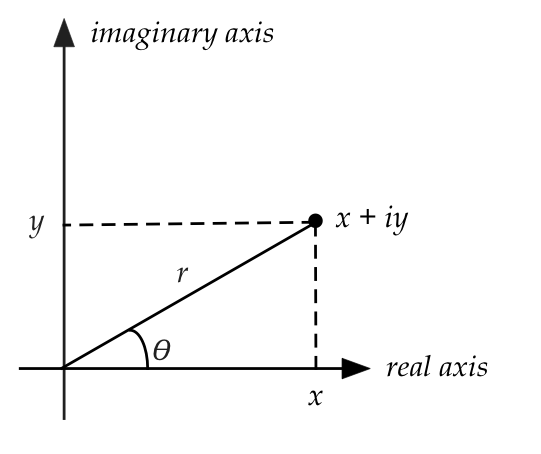
\includegraphics[width=3in]{notes/figs/n04/03complexnumber.png}
        \caption{Complex number distance from the origin}
        \label{fig:03complexnumber2}
    \end{figure}
    
    Note: $a^{2}+b^{2} \neq(a+b i)(a+b i)$, But $a^{2}+b^{2}=(a+b i)(a-b i)$. What does this have to do with the dot-product? For real vectors,
    
    $$
    \begin{aligned}
    \mathbf{u} \cdot \mathbf{u} &=\left(u_{1}, u_{2}, \ldots, u_{n}\right) \cdot\left(u_{1}, u_{2}, \ldots, u_{n}\right) \\
    &=u_{1}^{2}+u_{2}^{2}+\ldots+u_{n}^{2} \\
    &=\left|u_{1}\right|^{2}+\left|u_{2}\right|^{2}+\ldots+\left|u_{n}\right|^{2} \\
    &=|\mathbf{u}|^{2}
    \end{aligned}
    $$
    
    To make this work for complex numbers:
    
    $$
    \begin{aligned}
    \mathbf{u} \cdot \mathbf{u} &=\left(u_{1}^{*}, u_{2}^{*}, \ldots, u_{n}^{*}\right) \cdot\left(u_{1}, u_{2}, \ldots, u_{n}\right) \\
    &=u_{1}^{*} u_{1}+u_{2}^{*} u_{2}+\ldots+u_{n}^{*} u_{n} \\
    &=\left|u_{1}\right|^{2}+\left|u_{2}\right|^{2}+\ldots+\left|u_{n}\right|^{2} \\
    &=|\mathbf{u}|^{2}
    \end{aligned}
    $$
    
    inner product convention: Most math books use a different inner-product definition, where the right vector is conjugated:
    
    $$
    \mathbf{u} \cdot \mathbf{v}=u_{1} v_{1}^{*}+u_{2} v_{2}^{*}+\ldots+u_{n} v_{n}^{*}
    $$
    
    However, we will use the convention from physics, where the left vector is conjugated:
    
    $$
    \mathbf{u} \cdot \mathbf{v}=u_{1}^{*} v_{1}+u_{2}^{*} v_{2}+\ldots+u_{n}^{*} v_{n}
    $$
    
    Consider the complex numbers $u_{1}=(2+3 i)$ and $v_{1}=(3+4 i)$. Then
    
    $$
    \begin{aligned}
    &u_{1} v_{1}^{*}=(2+3 i)(3+4 i)^{*}=(2+3 i)(3-4 i)=(18+i) \\
    &u_{1}^{*} v_{1}=(2+3 i)^{*}(3+4 i)=(2-3 i)(3+4 i)=(18-i)
    \end{aligned}
    $$
    
    So, the definitions will result in different inner-products but $\mathbf{u} \cdot \mathbf{u}=|\mathbf{u}|^{2}$ still holds, and the real part is the same. The convention in physics and quantum computing is to left-conjugate, and that is what we will do. Incidentally, did you notice that in the above example $u_{1} v_{1}^{*}=\left(u_{1}^{*} v_{1}\right)^{*}$ ?

\subsection{Complex vectors (again) with Dirac notation}

    Let's first revisit two aspects of real vectors: 1. Symbolic convention: Most linear algebra textbooks use boldface or arrow notation for vectors as in:
    
    $$
    \mathbf{u}=\left[\begin{array}{r}
    1 \\
    2+i \\
    3 i
    \end{array}\right] \quad \vec{v}=\left[\begin{array}{l}
    2 \\
    1 \\
    i
    \end{array}\right]
    $$
    
    These are typically subscripted for multiple related vectors, as in:
    
    $$
    \mathbf{w}_{1}=\left[\begin{array}{r}
    1 \\
    -2 \\
    3
    \end{array}\right] \quad \mathbf{w}_{2}=\left[\begin{array}{l}
    2 \\
    0 \\
    1
    \end{array}\right]
    $$
    
    2. Dot product: The dot product for real vectors is, not surprisingly, written with a dot:
    
    $$
    \mathbf{w}_{1} \cdot \mathbf{w}_{2}=\left[\begin{array}{r}
    1 \\
    -2 \\
    3
    \end{array}\right] \cdot\left[\begin{array}{l}
    2 \\
    0 \\
    1
    \end{array}\right]=5
    $$
    
    The result is a number. We can treat each real vector as a single-column matrix and instead write the dot-product as:
    
    $$
    \mathbf{w}_{1}^{T} \mathbf{w}_{2}=\left[\begin{array}{lll}
    1 & -2 & 3
    \end{array}\right] \cdot\left[\begin{array}{l}
    2 \\
    0 \\
    1
    \end{array}\right]=5
    $$
    
    Here, with a slight abuse of notation, the $1 \times 1$ result can be interpreted as a number. Note: for a complex vector, we'll need to both transpose and conjugate the left vector:
    
    $$
    \begin{aligned}
    \mathbf{u} \cdot \mathbf{v} &=\left(\mathbf{u}^{*}\right)^{T} \mathbf{v} \\
    &=\left(\left[\begin{array}{c}
    1 \\
    (2-i) \\
    3 i
    \end{array}\right]^{*}\right)^{T}\left[\begin{array}{l}
    2 \\
    1 \\
    i
    \end{array}\right] \\
    &=\left(\left[\begin{array}{c}
    1 \\
    (2+i) \\
    -3 i
    \end{array}\right]\right)^{T}\left[\begin{array}{l}
    2 \\
    1 \\
    i
    \end{array}\right] \\
    &=\left[\begin{array}{lll}
    1 & (2+i) & -3 i]
    \end{array}\right]\left[\begin{array}{l}
    2 \\
    1 \\
    i
    \end{array}\right] \\
    &=7+i
    \end{aligned}
    $$
    
    We could have transposed first and then conjugated:
    
    $$
    \begin{aligned}
    \left(\mathbf{u}^{*}\right)^{T} \mathbf{v} &=\left(\left[\begin{array}{c}
    1 \\
    (2-i) \\
    3 i
    \end{array}\right]^{T}\right)^{*}\left[\begin{array}{l}
    2 \\
    1 \\
    i
    \end{array}\right] \\
    &=\left(\left[\begin{array}{lll}
    1 & (2-i) & 3 i
    \end{array}\right)^{*}\left[\begin{array}{l}
    2 \\
    1 \\
    i
    \end{array}\right]\right.\\
    &=\left[\begin{array}{lll}
    1 & (2+i) & -3 i
    \end{array}\right]\left[\begin{array}{l}
    2 \\
    1 \\
    i
    \end{array}\right] \\
    &=7+i
    \end{aligned}
    $$
    
    The first thing to do is to invent notation for combined transpose and conjugation: the dagger notation
    
    $$
    \mathbf{u}^{\dagger}=\left[u_{1}^{*} \ldots u_{n}^{*}\right]
    $$
    
    Then, we can write
    
    $$
    \left(\mathbf{u}^{*}\right)^{T} \mathbf{v}=\left(\mathbf{u}^{T}\right)^{*} \mathbf{v}=\mathbf{u}^{\dagger} \mathbf{v}
    $$
    
    Now on to Dirac notation for vectors: A column vector is written as in these examples:
    
    $$
    |v\rangle=\left[\begin{array}{c}
    2 \\
    1 \\
    i
    \end{array}\right]
    $$
    $$
    |u\rangle=\left[\begin{array}{c}
    1 \\
    (2-i) \\
    3 i
    \end{array}\right]
    $$
    
    A conjugated row vector is written as 
    
    $$
    \langle u|=(|u\rangle)^{\dagger}=\left[\begin{array}{ccc}
    1^{*} & (2-i)^{*} & (3 i)^{*}
    \end{array}\right]=\left[\begin{array}{lll}
    1 & 2+i & -3 i
    \end{array}\right]
    $$
    
    And, most crucially, the dot product of $|u\rangle$ and $|v\rangle$ is shown in Figure \ref{fig:05dirac2}.
    
    \begin{figure}
        \centering
        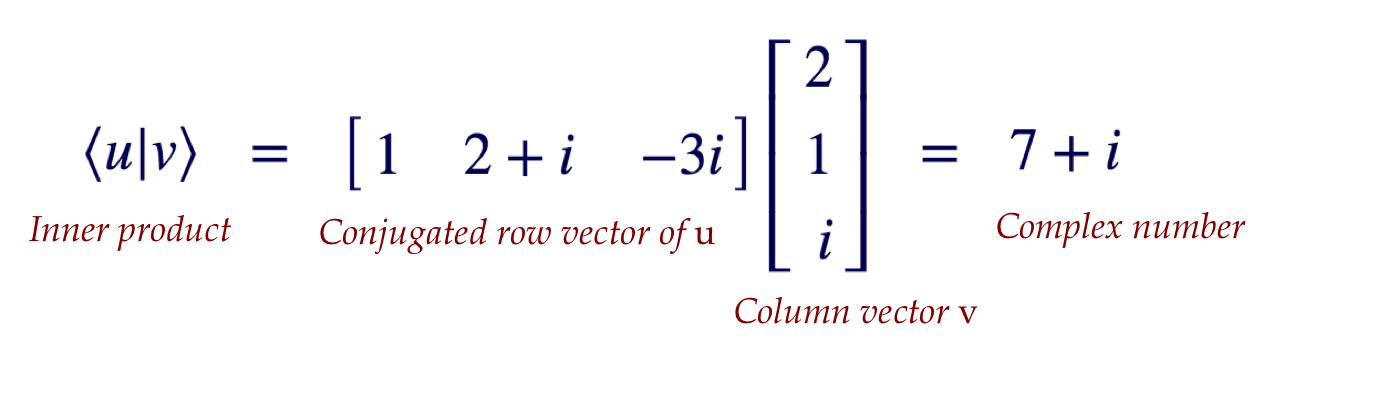
\includegraphics[width=5in]{notes/figs/n04/05dirac2.png}
        \caption{Inner product, conjugated row vector of u, column vector v, complex number}
        \label{fig:05dirac2}
    \end{figure}
    
    Symbolically for general vectors $|u\rangle=\left(u_{1}, \ldots, u_{n}\right)$ and $|v\rangle=\left(v_{1}, \ldots, v_{n}\right)$,
    
    $$
    \langle u \mid v\rangle=\sum_{i} u_{i}^{*} v_{i}
    $$
    
    This is also commonly called the inner product. Next, we'll use the same notation to write an outer product shown in Figure \ref{fig:06dirac3}.
    
    \begin{figure}
        \centering
        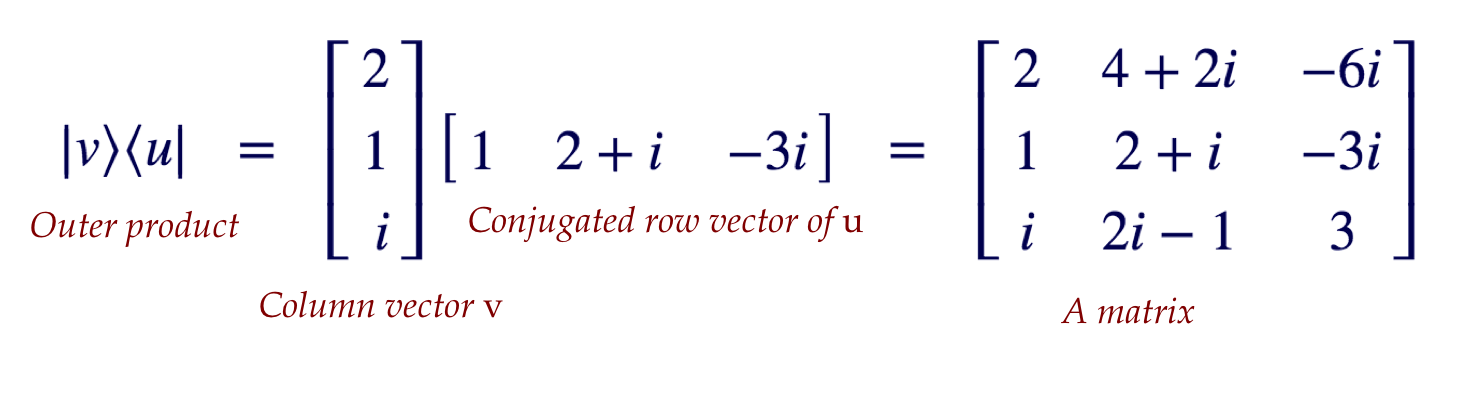
\includegraphics[width=5in]{notes/figs/n04/06dirac3.png}
        \caption{Outer product, column vector $v$, Conjugated row vector of $u$, A matrix}
        \label{fig:06dirac3}
    \end{figure}
    
    This can be summarized in Figure \ref{fig:07dirac}.
    
    \begin{figure}
        \centering
        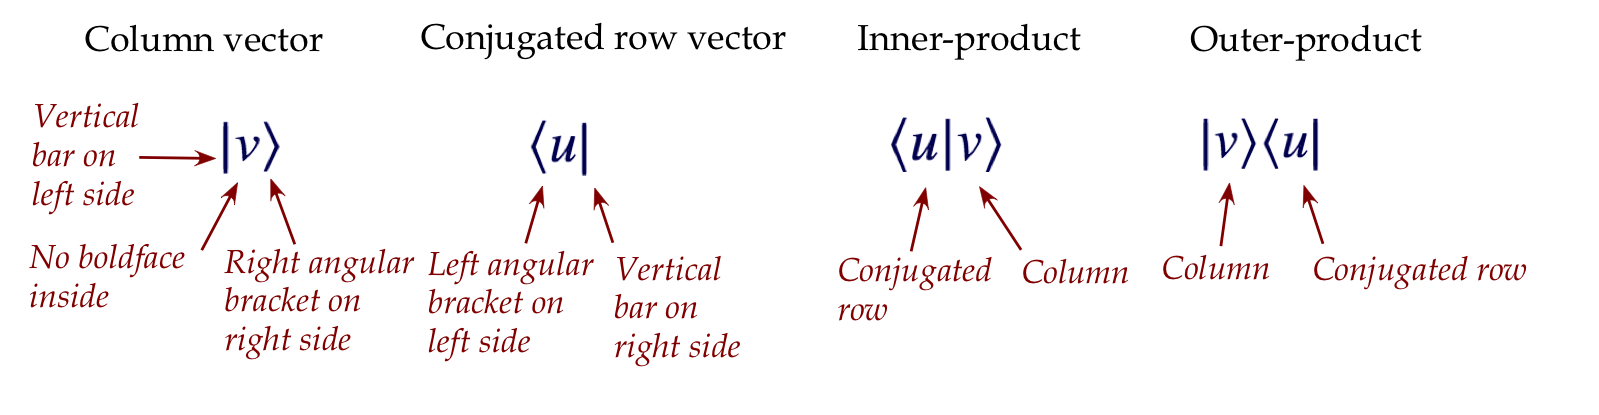
\includegraphics[width=5in]{notes/figs/n04/07dirac.png}
        \caption{Column vector, Conjugated row vector, Inner-product, Outer-product}
        \label{fig:07dirac}
    \end{figure}
    
    One needs to be careful with subscripts: In traditional notation, we wrote a collection of vectors $\mathbf{u}_{1}, \mathbf{u}_{2}, \ldots, \mathbf{u}_{n}$ with subscripts not boldfaced. In Dirac notation, a collection of $n$ vectors is described as: $\left|u_{1}\right\rangle,\left|u_{2}\right\rangle, \ldots,\left|u_{n}\right\rangle$. The subscripts are inside the asymmetric brackets. Unfortunately, this can lead to confusion when we want to describe the individual numbers in a vector, as in: $|v\rangle=\left(v_{1}, v_{2}, \ldots, v_{n}\right)$. Thus, one needs to infer the correct meaning from the context. Scalars and scalar conjugation: First consider an example with real scalars and vectors:
    
    $$
    3\left[\begin{array}{r}
    1 \\
    -2 \\
    3
    \end{array}\right]=\left[\begin{array}{r}
    3 \\
    -6 \\
    9
    \end{array}\right]
    $$
    
    Note: The result is the same in row form:
    
    $$
    3\left[\begin{array}{lll}
    1 & -2 & 3
    \end{array}\right]=\left[\begin{array}{lll}
    3 & -6 & 9
    \end{array}\right]
    $$
    
    Symbolically, if $\mathbf{w}=\left(w_{1}, w_{2}, \ldots, w_{n}\right)$ is a real vector and $\alpha$ is a real number, then:
    
    $$
    (\alpha \mathbf{w})^{T}=\alpha \mathbf{w}^{T}
    $$
    
    In our example:
    
    $$
    \left(3\left[\begin{array}{r}
    1 \\
    -2 \\
    3
    \end{array}\right]\right)^{T}=3\left[\begin{array}{lll}
    1 & -2 & 3
    \end{array}\right]
    $$
    
    But, because we conjugate complex vectors when transposing, the scalar can get conjugated. Let's first look at this symbolically: Suppose $|w\rangle=\left(w_{1}, \ldots, w_{n}\right)$ is a complex vector and $\alpha$ a complex number. Then we'll use the notation $|\alpha w\rangle$ to mean
    
    $$
    |\alpha w\rangle=\left[\begin{array}{r}
    \alpha w_{1} \\
    \vdots \\
    \alpha w_{n}
    \end{array}\right]=\alpha\left[\begin{array}{r}
    w_{1} \\
    \vdots \\
    w_{n}
    \end{array}\right]=\alpha|w\rangle
    $$
    
    where $\alpha$ multiplies into each number in the vector. In contrast, observe that
    
    $$
    \begin{aligned}
    \langle\alpha w| &=\left[\begin{array}{lll}
    \left(\alpha w_{1}\right) & \cdots & \left(\alpha w_{n}\right)
    \end{array}\right]^{*} \\
    &=\left[\begin{array}{lll}
    \left(\alpha w_{1}\right)^{*} & \cdots & \left(\alpha w_{n}\right)^{*}
    \end{array}\right] \\
    &=\left[\begin{array}{lll}
    \alpha^{*} w_{1}^{*} & \cdots & \alpha^{*} w_{n}^{*}
    \end{array}\right] \\
    &=\alpha^{*}\left[\begin{array}{lll}
    w_{1}^{*} & \cdots & w_{n}^{*}
    \end{array}\right] \\
    &=\alpha^{*}\langle w|
    \end{aligned}
    $$
    
    Thus, when a scalar is factored out of a conjugated-row, the scalar becomes conjugated. An example: Suppose
    
    $$
    \alpha=(2-3 i), \quad|w\rangle=\left[\begin{array}{r}
    1 \\
    -2 \\
    3
    \end{array}\right]
    $$
    
    Then, in this case
    
    $$
    \langle w|=\left[\begin{array}{lll}
    1 & -2 & 3
    \end{array}\right]
    $$
    
    (The conjugate of a real number is the same real number.) Next,
    
    $$
    \alpha|w\rangle=(2-3 i)\left[\begin{array}{r}
    1 \\
    -2 \\
    3
    \end{array}\right]=\left[\begin{array}{r}
    2-3 i \\
    -4+6 i \\
    6-9 i
    \end{array}\right]
    $$
    
    That is, the scalar multiplies each element in the usual way. If we conjugate and transpose the result, we get
    
    $$
    (\alpha|w\rangle)^{\dagger}=\left(\left[\begin{array}{r}
    2-3 i \\
    -4+6 i \\
    6-9 i
    \end{array}\right]\right)^{\dagger}=\left[\begin{array}{lll}
    2+3 i & -4-6 i & 6+9 i
    \end{array}\right]
    $$
    
    which is NOT equal to $(2-3 i)\left[\begin{array}{lll}1 & -2 & 3\end{array}\right]$, i.e., not equal to $\alpha\langle w|$ But
    
    $$
    \left[\begin{array}{lll}
    2+3 i & -4-6 i & 6+9 i
    \end{array}\right]=(2+3 i)\left[\begin{array}{ccc}
    1 & -2 & 3
    \end{array}\right]=\alpha^{*}\langle w|
    $$
    
    That is,
    
    $$
    (\alpha|w\rangle)^{\dagger}=\alpha^{*}\langle w|
    $$
    
    Lastly, for the magnitude of a vector $|u\rangle$, note that
    
    $$
    || u\rangle\left.\right|^{2}=\langle u \mid u\rangle
    $$
    
    Why? Recall: that's how we arrived at the definition of inner product! When the context makes it clear, we'll simplify the magnitude notation to $|u|$. Vector operations: We've already seen scalar multiplication and inner product. The only other operation needed is plain old addition, which is the same as in real vectors, for example:
    
    $$
    \left[\begin{array}{l}
    2 \\
    1 \\
    i
    \end{array}\right]+\left[\begin{array}{r}
    1 \\
    -2 \\
    3
    \end{array}\right]=\left[\begin{array}{r}
    3 \\
    -1 \\
    3+i
    \end{array}\right]
    $$
    
    Notationally, we write this in two equivalent ways:
    
    $$
    |v+w\rangle \triangleq|v\rangle+|w\rangle
    $$
    
    Note: The right side is easy: it's merely element-by-element addition of two vectors to give a third. The left side is a bit strange because we haven't said anything about what $v+w$ means inside the Dirac brackets. The above definition clarifies. Scalar "movement": There is a type of algebraic simplification we often see in quantum computing that's worth highlighting. We'll do so with real vector examples, but the same idea applies to complex vectors. Consider $|v\rangle=(3,1)$ and $\alpha=5$ : We typically write the scalar multiplication as: $5\left[\begin{array}{l}3 \\ 1\end{array}\right]$ We could just as correctly write it as:
    
    $$
    \left[\begin{array}{l}
    3 \\
    1
    \end{array}\right] 5
    $$
    
    In this sense, the scalar is "movable" when applied as a multiplier.
    
    This matters when the scalar itself comes as a result of an inner product. For example, suppose $|u\rangle=(1,2),|v\rangle=(3,1)$ : Then, consider the outer-product (matrix) $|v\rangle\langle v|$ times the vector $|u\rangle$ :
    
    $$
    \begin{aligned}
    (|v\rangle\langle v|)|u\rangle &=\left(\left[\begin{array}{l}
    3 \\
    1
    \end{array}\right]\left[\begin{array}{ll}
    3 & 1
    \end{array}\right]\right)\left[\begin{array}{l}
    1 \\
    2
    \end{array}\right] \\
    &=\left(\left[\begin{array}{ll}
    9 & 3 \\
    3 & 1
    \end{array}\right]\right)\left[\begin{array}{l}
    1 \\
    2
    \end{array}\right] \\
    &=\left[\begin{array}{r}
    15 \\
    5
    \end{array}\right]
    \end{aligned}
    $$
    
    Instead, observe that we can do this differently by exploiting matrix-associativity:
    
    $$
    \begin{aligned}
    (|v\rangle\langle v|)|u\rangle &=|v\rangle(\langle v \mid u\rangle) \\
    &=\left[\begin{array}{l}
    3 \\
    1
    \end{array}\right]([3\\
    &=\left[\begin{array}{l}
    3 \\
    1
    \end{array}\right](5) \\
    &=5\left[\begin{array}{l}
    3 \\
    1
    \end{array}\right] \\
    &=\left[\begin{array}{r}
    15 \\
    5
    \end{array}\right]
    \end{aligned}
    $$
    
    Symbolically, a movable scalar might represent an inner-product, which when moved, results in simplification:
    
    $$
    (|v\rangle\langle v|)|u\rangle=|v\rangle(\langle v \mid u\rangle)=(\langle v \mid u\rangle)|v\rangle
    $$
    
    Linear combinations: Combining scalar multiplication and addition gives us a linear combination, and some notation for it:
    
    $$
    |\alpha u+\beta v\rangle \triangleq \alpha|u\rangle+\beta|v\rangle
    $$
    
    For conjugated rows, we need to conjugate the scalars:
    
    $$
    \langle\alpha u+\beta v| \triangleq \alpha^{*}\langle u|+\beta^{*}\langle v|
    $$
    
    This leads to two forms of inner products with linear combinations: $\langle u \mid \alpha v+\beta w\rangle=\alpha\langle u \mid v\rangle+\beta\langle u \mid w\rangle \quad$ Linearity on the right
    $\langle\alpha u+\beta v \mid w\rangle=\alpha^{*}\langle u \mid w\rangle+\beta^{*}\langle v \mid w\rangle \quad$ Conjugate linearity on the left Both are important to remember! How to read the notation $|\alpha u+\beta v\rangle$ : First start with $u$ and $v$ as regular column vectors, as in
    
    $$
    |u\rangle=\left[\begin{array}{r}
    1 \\
    2-i \\
    3 i
    \end{array}\right] \quad|v\rangle=\left[\begin{array}{l}
    2 \\
    1 \\
    i
    \end{array}\right]
    $$
    
    Then compute the column vector $\alpha u+\beta v$, for example with $\alpha=(2-3 i), \beta=-1$ :
    
    $$
    \alpha u+\beta v=(2-3 i)\left[\begin{array}{r}
    1 \\
    2-i \\
    3 i
    \end{array}\right]+(-1)\left[\begin{array}{l}
    2 \\
    1 \\
    i
    \end{array}\right]=\left[\begin{array}{r}
    -3 i \\
    -8 i \\
    9+5 i
    \end{array}\right]
    $$
    
    This is already a column, so we can write it as

    $$
    |\alpha u+\beta v\rangle=\left[\begin{array}{r}
    -3 i \\
    -8 i \\
    9+5 i
    \end{array}\right]
    $$
    
    How to read the notation $\langle\alpha u+\beta v|$ : First think of $\alpha u+\beta v$ as the column
    
    $$
    \alpha u+\beta v=\left[\begin{array}{r}
    -3 i \\
    -8 i \\
    9+5 i
    \end{array}\right]
    $$
    
    Now conjugate and transpose:
    
    $$
    \langle\alpha u+\beta v|=\left[\begin{array}{lll}
    3 i & 8 i \quad 9-5 i
    \end{array}\right]
    $$
    
    Important: The above notation for linear combinations is worth re-reading several times: we will use this frequently throughout the course. Conjugating and transposing a matrix: Just as the "dagger" transposes and conjugates a vector, the same can be applied to a matrix. For example: Let
    
    $$
    A=\left[\begin{array}{cc}
    1+i & -i \\
    i & 1+1
    \end{array}\right]
    $$
    
    Then the transpose is
    
    $$
    A^{T}=\left[\begin{array}{cc}
    1+i & i \\
    -i & 1+i
    \end{array}\right]
    $$
    
    And the conjugate of the transpose is:
    
    $$
    A^{\dagger}=\left(A^{T}\right)^{*}=\left[\begin{array}{cc}
    1-i & -i \\
    i & 1-i
    \end{array}\right]
    $$
    
    The matrix $A^{\dagger}$ is called the adjoint of $A$.
    
\subsection{Vector spaces, spans, bases, dimension, orthogonality}

    We're already familiar with these from prior linear algebra but let's do a quick review using Dirac notation. In the definitions below, we assume that the vectors in any set have the same number of elements: It is never the case that we want to put, for example, $(1,-2,3)$ and $(5,6)$ in the same set.
    Definitions: Span. Given a collection of vectors $\left|v_{1}\right\rangle,\left|v_{2}\right\rangle, \ldots,\left|v_{k}\right\rangle$, the span of these vectors is the set of all possible linear combinations of these (with complex scalars):
    
    $$
    \operatorname{span}\left(\left|v_{1}\right\rangle,\left|v_{2}\right\rangle, \ldots,\left|v_{k}\right\rangle\right) \triangleq\left\{\alpha_{1}\left|v_{1}\right\rangle+\alpha_{2}\left|v_{2}\right\rangle+\ldots+\alpha_{k}\left|v_{k}\right\rangle: \alpha_{i} \in \mathbb{C}\right\}
    $$
    
    Note: just like $\mathbb{R}$ is the set of all real numbers, we use $\mathbb{C}$ for the set of all complex numbers. Vector space. A vector space $V$ is a set of vectors such that, for any subset $\left|v_{1}\right\rangle,\left|v_{2}\right\rangle, \ldots,\left|v_{k}\right\rangle$ where $\left|v_{i}\right\rangle \in V$,
    
    $$
    \operatorname{span}\left(\left|v_{1}\right\rangle,\left|v_{2}\right\rangle, \ldots,\left|v_{k}\right\rangle\right) \subseteq V
    $$
    
    Think of a vector space as: it contains all the linear combinations of anything inside it. The special vector space $\mathbb{C}^{n}$ :
    
    $$
    \mathbb{C}^{n}=\left\{|v\rangle=\left(v_{1}, \ldots, v_{n}\right): v_{i} \in \mathbb{C}\right\}
    $$
    
    That is, the set of all vectors with $n$ elements, where each element is a complex number. Thus, for example, $(1,2+i, 3 i) \in \mathbb{C}^{3}$. And $(1,0,1,1,0) \in \mathbb{C}^{5}$. Note: $\mathbb{C}^{3}$ is not a subset of $\mathbb{C}^{5}$. Linear independence. A collection of vectors $\left|v_{1}\right\rangle,\left|v_{2}\right\rangle, \ldots,\left|v_{k}\right\rangle$ is linearly independent if
    
    $$
    \alpha_{1}\left|v_{1}\right\rangle+\alpha_{2}\left|v_{2}\right\rangle+\ldots+\alpha_{k}\left|v_{k}\right\rangle=0
    $$
    
    implies $\forall i: \alpha_{i}=0$. Basis. There are multiple equivalent definitions: 1. A basis for a given vector space $V$, is a set of vectors $\left|v_{1}\right\rangle,\left|v_{2}\right\rangle, \ldots,\left|v_{n}\right\rangle$ from $V$ such that: i. $\left|v_{1}\right\rangle,\left|v_{2}\right\rangle, \ldots,\left|v_{n}\right\rangle$ are linearly independent. ii. $V=\operatorname{span}\left(\left|v_{1}\right\rangle,\left|v_{2}\right\rangle, \ldots,\left|v_{n}\right\rangle\right)$ 2. A basis for a given vector space $V$, is a set of vectors $\left|v_{1}\right\rangle,\left|v_{2}\right\rangle, \ldots,\left|v_{n}\right\rangle$ from $V$ such that any vector $|u\rangle \in V$ is uniquely expressible as a linear combination of the $\left|v_{i}\right\rangle$ 's. That is, there is only one linear combination $|u\rangle=\sum_{i} \alpha_{i}\left|v_{i}\right\rangle$. Note: all bases have the same number of vectors. That is, if one basis has $n$ vectors, so does any other basis. Dimension. The dimension of a vector space $V$ is the number of vectors in any basis, written as $\operatorname{dim}(V)$. As a consequence, if $\operatorname{dim}(V)=n$, any $n$ linearly independent vectors from $V$ forms a basis for $V$. Orthogonal vectors. Two vectors $|u\rangle$ and $|v\rangle$ from a vector space $V$ are orthogonal if $\langle u \mid v\rangle=0$. Note: if $\langle u \mid v\rangle=0$, then $\langle v \mid u\rangle=0$. Orthonormal vectors. Two vectors $|u\rangle$ and $|v\rangle$ from a vector space $V$ are orthonormal if $\langle u \mid v\rangle=0$ and $|u|=|v|=1$ (that is, each is of unit length). Orthonormal basis. An orthonormal basis $\left|v_{1}\right\rangle,\left|v_{2}\right\rangle, \ldots,\left|v_{n}\right\rangle$ for a vector space $V$ is a basis such that $\left\langle v_{i} \mid v_{j}\right\rangle=0$ and $\left\langle v_{i} \mid v_{i}\right\rangle=1$.
    
    Expressing a vector in an orthonormal basis: If $\left|v_{1}\right\rangle,\left|v_{2}\right\rangle, \ldots,\left|v_{n}\right\rangle$ is an orthonormal basis for $V$, and $|u\rangle \in V$ is expressed as
    
    $$
    |u\rangle=\alpha_{1}\left|v_{1}\right\rangle+\ldots+\alpha_{n}\left|v_{n}\right\rangle
    $$
    
    then it's easy to calculate each coefficient $\alpha_{i}$ as
    
    $$
    \alpha_{i}=\left\langle v_{i} \mid u\right\rangle
    $$
    
    It's worth examining why: 
    
    $$
    \begin{aligned}\left\langle v_{i} \mid u\right\rangle &=\left\langle v_{i} \mid \alpha_{1} v_{1}+\alpha_{2} v_{2} \ldots+\ldots+\alpha_{n} v_{n}\right\rangle & & \text { Erpand }|u\rangle \\ &=\alpha_{1}\left\langle v_{i} \mid v_{1}\right\rangle+\alpha_{2}\left\langle v_{i} \mid v_{2}\right\rangle+\ldots+\alpha_{n}\left\langle v_{i} \mid v_{n}\right\rangle & & \text { Right-linearity of imner-product } \\ &=\alpha_{i}\left\langle v_{i} \mid v_{i}\right\rangle & & \text { All others are 0 } \\ &=\alpha_{i}\left|v_{i}\right|^{2} & & \\ &=\alpha_{i} & & \text { All }\left|v_{i}\right\rangle \text { 's are unit length } \end{aligned}
    $$

    All $\left|v_{t}\right\rangle^{\prime}$ s are unit length. Note: all but one of the inner products are zero. Some terminology: Writing a vector as a linear combination of basis vectors
    
    $$
    |u\rangle=\alpha_{1}\left|v_{1}\right\rangle+\ldots+\alpha_{n}\left|v_{n}\right\rangle
    $$
    
    is called expanding a vector in a basis. The complex scalars $\alpha_{i}$ are called coefficients or amplitudes. What's important to know about vectors and bases in quantum computing: Nearly all vectors encountered will be unit vectors (magnitude $=1$ ). When an exception occurs, we typically normalize the vector to make it unit-length:
    
    $$
    |v\rangle=\frac{1}{|u|}|u\rangle
    $$
    
    Nearly all bases will be orthonormal bases. These properties simplify expressions and calculations but at first can be a bit confusing. 
    
    The standard basis for $\mathbb{C}^{n}$ : Define the $n$ vectors $\left|e_{1}\right\rangle, \ldots,\left|e_{n}\right\rangle$ where $\left|e_{i}\right\rangle=(0,0, \ldots, 1, \ldots, 0)$ D All $0^{\prime}$ s with a 1 as the i-th element. Example: for $\mathbb{C}^{3}$ :
    
    $$
    \left|e_{1}\right\rangle=\left[\begin{array}{l}
    1 \\
    0 \\
    0
    \end{array}\right] \quad\left|e_{2}\right\rangle=\left[\begin{array}{l}
    0 \\
    1 \\
    0
    \end{array}\right] \quad\left|e_{3}\right\rangle=\left[\begin{array}{l}
    0 \\
    0 \\
    1
    \end{array}\right]
    $$
    
    This basis is often called the standard basis and sometimes the computational basis. Note: the standard basis itself has no complex numbers. Any complex vector is nonetheless expressible via complex coefficients. We'll shortly see a somewhat unusual but commonly used notation for the standard basis.
    
\subsection{More about Dirac notation}
    
    At this point you may be wondering why we bother with this "asymmetric" notation? There are four reasons. The first two are: The notation nicely tracks conjugation and transpose. For example, consider an outer-product matrix $|u\rangle\langle v|$ times a vector $|w\rangle$ as shown in Figure \ref{fig:08dirac4}.
    
    \begin{figure}
        \centering
        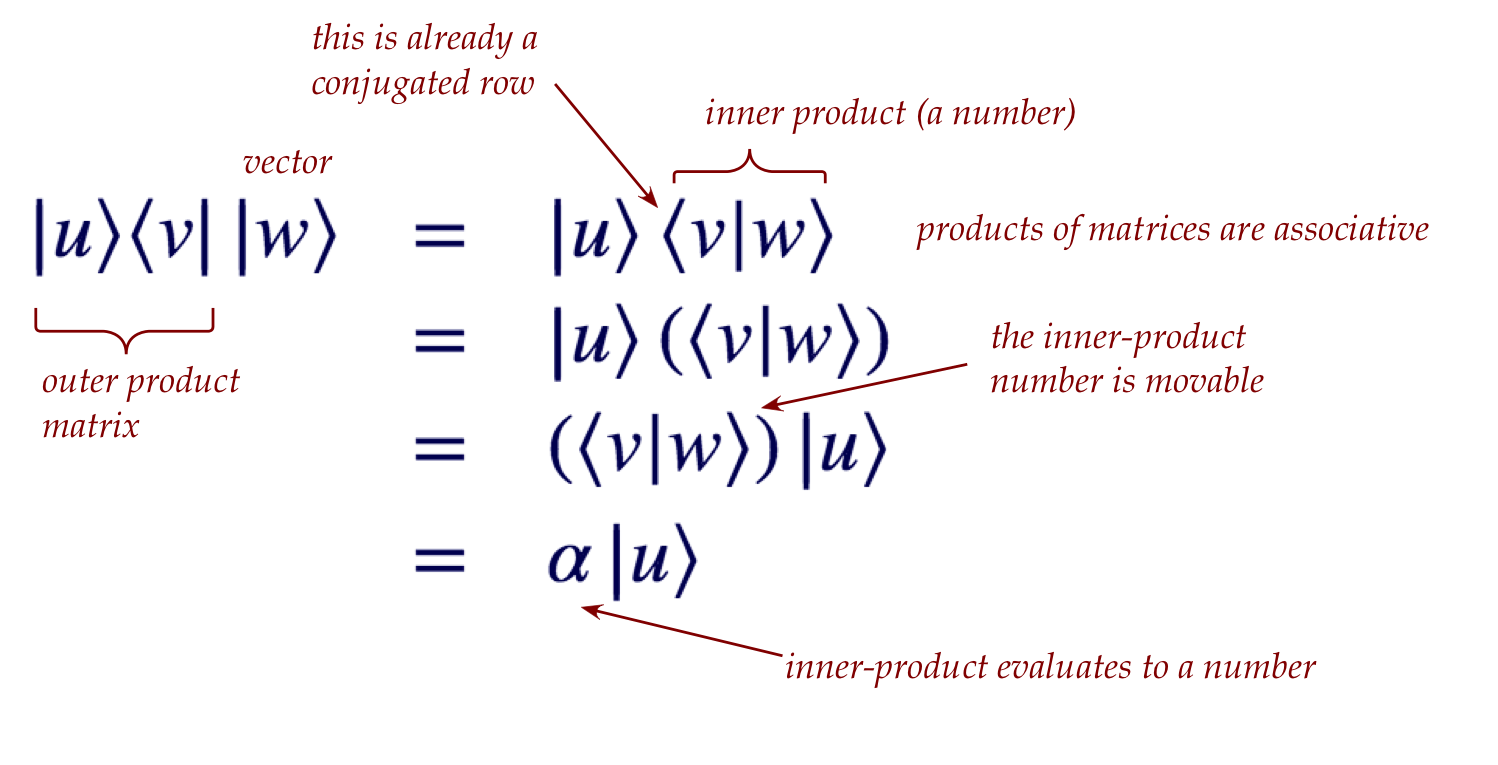
\includegraphics[width=5in]{notes/figs/n04/08dirac4.png}
        \caption{Outer product matrix times a vector}
        \label{fig:08dirac4}
    \end{figure}
    
    The asymmetric brackets make the conjugation status obvious. Because the brackets delineate a single vector, one can write something more elaborate in between as in: |3rd qubit $\rangle$, $\langle A u|$, where the operator $A$ is applied to the vector $u$ and then the result is turned into a conjugated row. We'll now get to the third reason, which is that a convention has been developed with the notation that greatly eases descriptions for quantum computing: Let's start with the standard basis for $\mathbb{C}^{2}:(1,0)$ and $(0,1)$. These are named in Dirac notation as $|0\rangle \triangleq\left[\begin{array}{l}1 \\ 0\end{array}\right]$, $|1\rangle \triangleq\left[\begin{array}{l}0 \\ 1\end{array}\right]$. Well later see that these will correspond to two special states of a single qubit. Note: The vector $|0\rangle$ is not the zero vector. The next larger size is two qubits, with four states and four standard-basis vectors: 
    
    $$
    |00\rangle \triangleq\left[\begin{array}{l}1 \\ 0 \\ 0 \\ 0\end{array}\right] \quad|01\rangle \triangleq\left[\begin{array}{l}0 \\ 1 \\ 0 \\ 0\end{array}\right] \quad|10\rangle \triangleq\left[\begin{array}{l}0 \\ 0 \\ 1 \\ 0\end{array}\right] \quad|11\rangle \triangleq\left[\begin{array}{l}0 \\ 0 \\ 0 \\ 1\end{array}\right]
    $$
    
    Here are two 3-qubit example states: $|10010001\rangle\langle 10010001|$. At the moment, this won't make sense but pay attention to the compactness of notation: If we go to 8 bits, the Dirac notation gives us vectors like $|10010001\rangle$. The same vector in standard column form will have $2^{8}=256$ numbers! The problem gets worse once we have expressions that combine such vectors: For example, the outer product (a matrix) is written just like that. In conventional linear algebra, this is a $256 \times 256$ matrix. We will also have to get used to further shortcuts like these: Recall the four two-qubit vectors above: $|00\rangle,|01\rangle,|10\rangle,|11\rangle$. These are also often written as: $|0\rangle,|1\rangle,|2\rangle,|3\rangle$. Here, it's understood that the numbers $0,1,2,3$ are the decimal version of $00,01,10,11$. In this way, the three-qubit vectors from above get compactly written as: $|0\rangle,|1\rangle,|2\rangle,|3\rangle,|4\rangle,|5\rangle,|6\rangle,|7\rangle$. We will also need to get used to placing unusual symbols in this notation, for example: $\circ|+\rangle$ : Yes, that's the plus symbol in there, representing the vector $|+\rangle=\left(\frac{1}{\sqrt{2}}, \frac{1}{\sqrt{2}}\right)$. $|\uparrow\rangle$ : The "up arrow" represents vertical polarization (in a polarized light setting), as $|\rightarrow\rangle$ represents horizontal polarization. Other examples are: $|\nearrow\rangle$ and $|\nwarrow\rangle$ Think of these as alternatives to Greek-letter variable names. This can sometimes make for challenging reading as shown in Figure \ref{fig:09dirac7}.
    
    \begin{figure}
        \centering
        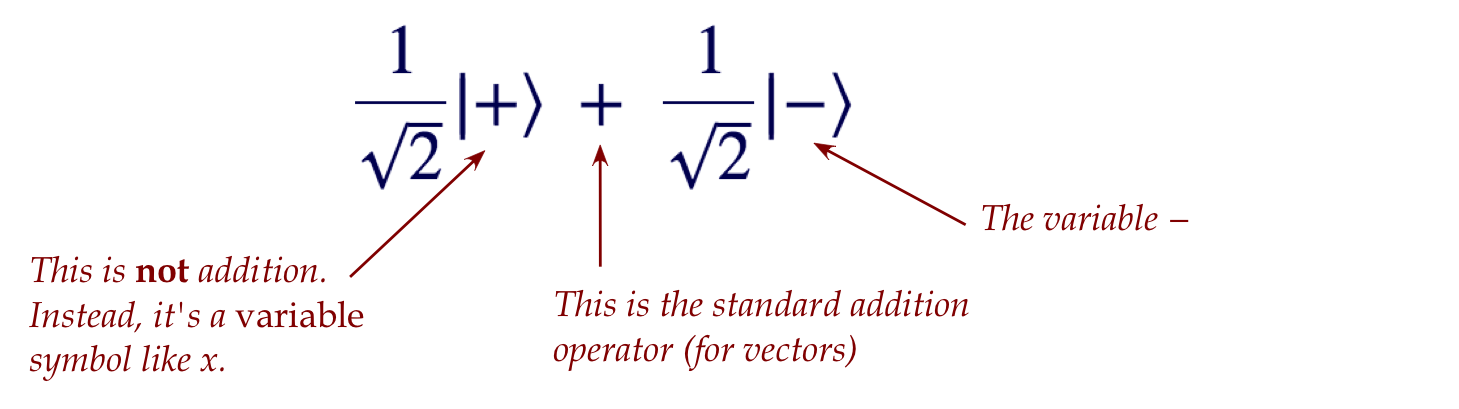
\includegraphics[width=5in]{notes/figs/n04/09dirac7.png}
        \caption{Challenging reading}
        \label{fig:09dirac7}
    \end{figure}
    
    This is a linear combination of the two vectors $|+\rangle$ and $|-\rangle$ Note: while conventional linear algebra likes to use letters like $u, v$, w for vectors, the quantum literature often uses $\psi$, pronounced "sigh". $\triangleright$ Thus, we will commonly see the notation $|\psi\rangle$. The fourth reason is valuable in quantum mechanics: It turns out that finite-sized vectors generalize to infinite-sized vectors quite easily: A regular vector like $|v\rangle=\left(v_{1}, v_{2}, \ldots, v_{n}\right)$ has its elements indexed by the integers $1,2, \ldots, n$. Then, when looking at $v_{i}$, the $i$ is an integer between 1 and $\mathrm{n}$. Think of the index $i$ as input, and the element $v_{i}$ as output shown in Figure \ref{fig:10dirac5}.
    
    \begin{figure}
        \centering
        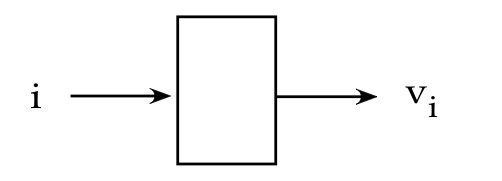
\includegraphics[width=2in]{notes/figs/n04/10dirac5.png}
        \caption{Index $i$ input and element $v_{i}$ as output}
        \label{fig:10dirac5}
    \end{figure}
    
    One could define vectors $|v\rangle=\left(v_{1}, v_{2}, \ldots\right)$ where the index set is all the natural numbers: $1,2,3, \ldots$. And one can define vectors with a real-valued index, where the elements are $v_{x}$. This is really nothing other than the function $v(x)$ shown in Figure \ref{fig:11dirac6}.
    
    \begin{figure}
        \centering
        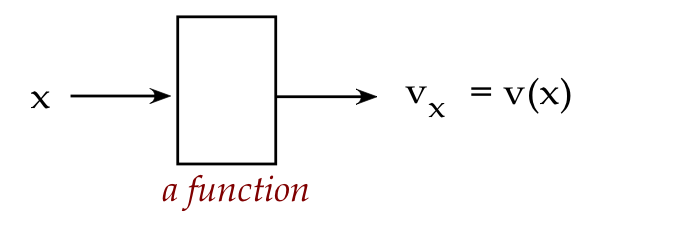
\includegraphics[width=2in]{notes/figs/n04/11dirac6.png}
        \caption{function $v(x)$}
        \label{fig:11dirac6}
    \end{figure}
    
    The Dirac notation is the same for functions: $|f(x)\rangle$. This fits in with the other kind of generalization that's needed when going from "finite and discrete" to "infinite and continuous": An operator is the equivalent generalization of a matrix. Again, Dirac notation treats both the same way, allowing for compact multi-use notation. Without knowing much more than we've just seen, we can already work with this notation: For example, consider the two vectors $|0\rangle=\left[\begin{array}{l}1 \\ 0\end{array}\right]$, $|1\rangle=\left[\begin{array}{l}0 \\ 1\end{array}\right]$. We can easily compute inner products:
    
    $$
    \begin{aligned}
    &\langle 0 \mid 0\rangle=\left[\begin{array}{ll}
    1 & 0
    \end{array}\right]\left[\begin{array}{l}
    1 \\
    0
    \end{array}\right]=1 \\
    &\langle 0 \mid 1\rangle=\left[\begin{array}{ll}
    1 & 0
    \end{array}\right]\left[\begin{array}{l}
    0 \\
    1
    \end{array}\right]=0 \\
    &\langle 1 \mid 0\rangle=\left[\begin{array}{ll}
    0 & 1
    \end{array}\right]\left[\begin{array}{l}
    1 \\
    0
    \end{array}\right]=0 \\
    &\langle 1 \mid 1\rangle=\left[\begin{array}{ll}
    0 & 1
    \end{array}\right]\left[\begin{array}{l}
    0 \\
    1
    \end{array}\right]=1
    \end{aligned}
    $$
    
    And outer products:
    
    $$
    \begin{aligned}
    &|0\rangle\langle 0|=\left[\begin{array}{l}
    1 \\
    0
    \end{array}\right]\left[\begin{array}{ll}
    1 & 0
    \end{array}\right]=\left[\begin{array}{ll}
    1 & 0 \\
    0 & 0
    \end{array}\right] \\
    &|0\rangle\langle 1|=\left[\begin{array}{l}
    1 \\
    0
    \end{array}\right]\left[\begin{array}{ll}
    0 & 1
    \end{array}\right]=\left[\begin{array}{ll}
    0 & 1 \\
    0 & 0
    \end{array}\right] \\
    &|1\rangle\langle 0|=\left[\begin{array}{l}
    0 \\
    1
    \end{array}\right]\left[\begin{array}{ll}
    1 & 0
    \end{array}\right]=\left[\begin{array}{ll}
    0 & 0 \\
    1 & 0
    \end{array}\right] \\
    &|1\rangle\langle 1|=\left[\begin{array}{l}
    0 \\
    1
    \end{array}\right]\left[\begin{array}{ll}
    0 & 1
    \end{array}\right]=\left[\begin{array}{ll}
    0 & 0 \\
    0 & 1
    \end{array}\right]
    \end{aligned}
    $$

\subsection{Projections and projectors}

    Because we don't have a convenient way to visualize a 2D complex vector, let's start with a description that uses real vectors as shown in Figure \ref{fig:11dirac6}.
    
    \begin{figure}
        \centering
        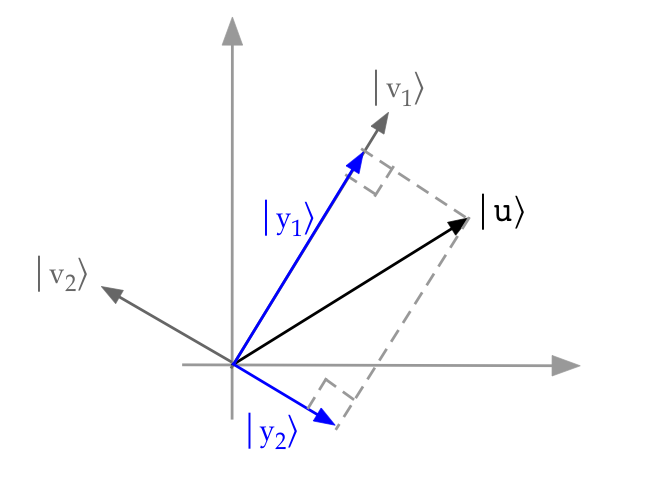
\includegraphics[width=3in]{notes/figs/n04/12projection.png}
        \caption{Visualize a 2D real vector}
        \label{fig:11dirac6}
    \end{figure}
    
    Here, $\left|v_{1}\right\rangle,\left|v_{2}\right\rangle$ are orthonormal basis vectors, and $|u\rangle$ is a vector. The picture shows the projection of $|u\rangle$ onto each of $\left|v_{1}\right\rangle$ and $\left|v_{2}\right\rangle$. Geometrically with real vectors, a projection is the shadow cast by one vector on another (with perpendicular light). For real vectors, we showed that
    
    $$
    \left|y_{1}\right\rangle=\left(\frac{\left\langle v_{1} \mid u\right\rangle}{\left\langle v_{1} \mid v_{1}\right\rangle}\right)\left|v_{1}\right\rangle
    $$
    
    When $\left|v_{1}\right\rangle,\left|v_{2}\right\rangle$ are unit-length, $\left\langle v_{i} \mid v_{i}\right\rangle=\left|v_{i}\right|^{2}=1$. Thus

    $$
    \left|y_{1}\right\rangle=\left\langle v_{1} \mid u\right\rangle\left|v_{1}\right\rangle
    $$

    Similarly
    
    $$
    \left|y_{2}\right\rangle=\left\langle v_{2} \mid u\right\rangle\left|v_{2}\right\rangle
    $$
    
    Most importantly, the two projections geometrically add up to the original vector:
    
    $$
    \begin{aligned}
    |u\rangle &=\left|y_{1}\right\rangle+\left|y_{2}\right\rangle \\
    &=\left\langle v_{1} \mid u\right\rangle\left|v_{1}\right\rangle+\left\langle v_{2} \mid u\right\rangle\left|v_{2}\right\rangle
    \end{aligned}
    $$
    
    What does a projection mean for complex vectors? Instead of thinking geometrically, we ll instead focus on this question: What parts of $\left|v_{1}\right\rangle,\left|v_{2}\right\rangle$ add up to $|u\rangle ?$ So, let's imagine (complex) numbers $\alpha_{1}, \alpha_{2}$ where

    $$
    \alpha_{1}\left|v_{1}\right\rangle+\alpha_{2}\left|v_{2}\right\rangle=|u\rangle
    $$

    We need to solve for the $\alpha^{\prime}$ s. Take the inner product with $\left|v_{1}\right\rangle$ on both sides: (Recall: the $v_{i}$ 's are orthonormal.) Thus, the coefficient-of-projection $\alpha_{i}$ is simply the inner product $\left\langle v_{i} \mid u\right\rangle$. In general, we'll have an orthonormal basis $\left|v_{1}\right\rangle,\left|v_{2}\right\rangle, \ldots,\left|v_{n}\right\rangle$, where for each for any vector $|u\rangle$ you have Figure \ref{fig:13projection2}.
    
    \begin{figure}
        \centering
        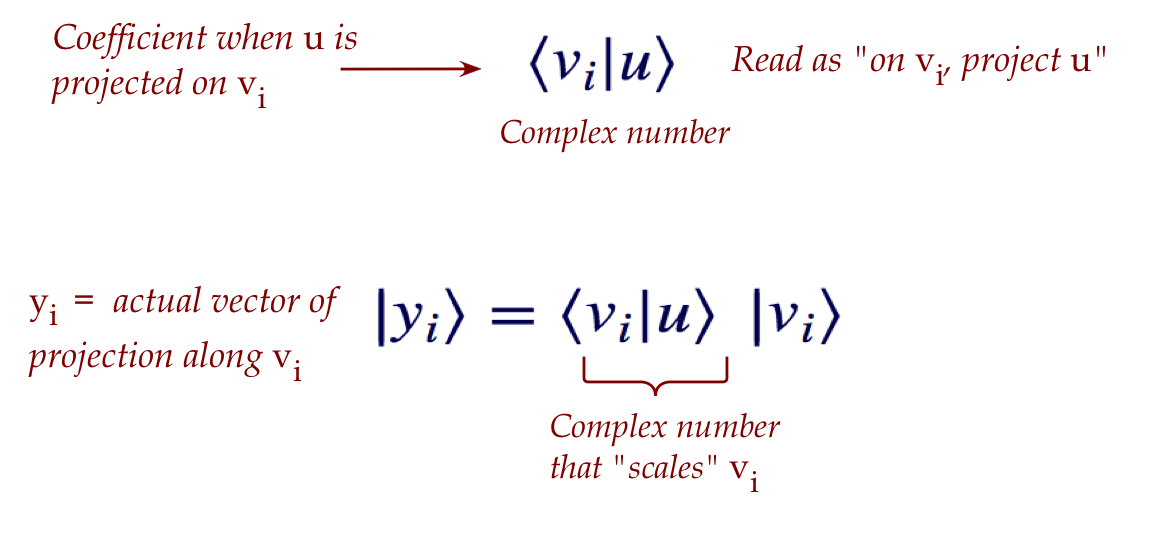
\includegraphics[width=4in]{notes/figs/n04/13projection2.png}
        \caption{Complex number that "scales" $v_i$}
        \label{fig:13projection2}
    \end{figure}
    
    Example: Suppose $|u\rangle=\left(\frac{\sqrt{3}}{2}, \frac{1}{2}\right)$ and $\left|v_{1}\right\rangle=\left(\frac{1}{2}, \frac{\sqrt{3}}{2}\right)$. Then,
    
    $$
    \begin{aligned}
    \left|y_{1}\right\rangle &=\left\langle v_{1} \mid u\right\rangle\left|v_{1}\right\rangle \\
    &=\left(\left[\begin{array}{cc}
    \frac{1}{2} & \frac{\sqrt{3}}{2}
    \end{array}\right]\left[\begin{array}{c}
    \frac{\sqrt{3}}{2} \\
    \frac{1}{2}
    \end{array}\right]\right)\left[\begin{array}{c}
    \frac{\sqrt{1}}{2} \\
    \frac{\sqrt{3}}{2}
    \end{array}\right]=\frac{\sqrt{3}}{2}\left[\begin{array}{c}
    \frac{1}{2} \\
    \frac{\sqrt{3}}{2}
    \end{array}\right]=\left[\begin{array}{c}
    \frac{\sqrt{3}}{4} \\
    \frac{1}{4}
    \end{array}\right]
    \end{aligned}
    $$
    
    Projectors or projection matrices: Now $\left|y_{1}\right\rangle$ is the vector that results from projecting the vector $|u\rangle$ on $\left|v_{1}\right\rangle$. We know that a matrix multiplying into a vector transforms it into another vector. Thus, one can ask: is there a matrix $P_{1}$ that would achieve this transformation, i.e.
    
    $$
    \left|y_{1}\right\rangle=P_{1}|u\rangle ?
    $$
    
    Such a matrix is called a projector matrix. Observe that
    
    $$
    \begin{aligned}
    \left|y_{1}\right\rangle &=\left(\left\langle v_{1} \mid u\right\rangle\right)\left|v_{1}\right\rangle & & \text { From earlier } \\
    &=\left|v_{1}\right\rangle\left(\left\langle v_{1} \mid u\right\rangle\right) & & \text { The scalar in parens can be moved } \\
    &=\left(\left|v_{1}\right\rangle\left\langle v_{1}\right|\right)|u\rangle & & \text { Associativity of matrix multiplication }
    \end{aligned}
    $$
    
    But we've seen that the outerproduct $\left|v_{1}\right\rangle\left\langle v_{1}\right|$ is in fact a matrix. So, let's define $P_{1} \triangleq\left|v_{1}\right\rangle\left\langle v_{1}\right|$. Note: $P_{1}$ depends only on the basis vector $\left|v_{1}\right\rangle$; it does not depend on $|u\rangle$. Just like we dropped boldface notation for vectors, we will do the same with matrices. Generally, we will use unbolded capital letters for matrices, (the convention in quantum computing/mechanics). It does take some getting used to. In our example:
    
    $$
    \left|v_{1}\right\rangle\left\langle v_{1}\right|=\left[\begin{array}{r}
    \frac{1}{2} \\
    \frac{\sqrt{3}}{2}
    \end{array}\right]\left[\begin{array}{ll}
    \frac{1}{2} & \frac{\sqrt{3}}{2}
    \end{array}\right]=\left[\begin{array}{cc}
    \frac{1}{4} & \frac{\sqrt{3}}{4} \\
    \frac{\sqrt{3}}{4} & \frac{3}{4}
    \end{array}\right] \triangleq P_{1}
    $$
    
    Then,
    
    $$
    P_{1}|u\rangle=\left[\begin{array}{cc}
    \frac{1}{4} & \frac{\sqrt{3}}{4} \\
    \frac{\sqrt{3}}{4} & \frac{3}{4}
    \end{array}\right]\left[\begin{array}{c}
    \frac{\sqrt{3}}{2} \\
    \frac{1}{2}
    \end{array}\right]=\left[\begin{array}{c}
    \frac{\sqrt{3}}{4} \\
    \frac{1}{4}
    \end{array}\right]=\left|y_{1}\right\rangle
    $$
    
    For our two-vector basis, the other projector is:
    
    $$
    P_{2}=\left|v_{2}\right\rangle\left\langle v_{2}\right|=\left[\begin{array}{c}
    \frac{-\sqrt{3}}{2} \\
    \frac{1}{2}
    \end{array}\right]\left[\begin{array}{ll}
    -\frac{\sqrt{3}}{2} & \frac{1}{2}
    \end{array}\right]=\left[\begin{array}{cc}
    \frac{3}{4} & -\frac{\sqrt{3}}{4} \\
    -\frac{\sqrt{3}}{4} & \frac{1}{4}
    \end{array}\right]
    $$
    
    The completeness relation for projectors: We'll explain the idea with a two-vector orthonormal basis $\left|v_{1}\right\rangle,\left|v_{2}\right\rangle$. First, we'll write $|u\rangle$ as the addition of $|u\rangle$ 's projections on $\left|v_{1}\right\rangle,\left|v_{2}\right\rangle$ :
    
    $$
    \begin{aligned}
    I|u\rangle &=|u\rangle \\
    &=P_{1}|u\rangle+P_{2}|u\rangle \\
    &=\left(P_{1}+P_{2}\right)|u\rangle
    \end{aligned}
    $$
    
    Thus
    $$
    \left(P_{1}+P_{2}-I\right)|u\rangle=\mathbf{0}
    $$
    
    for all $|u\rangle$. And so, the sum of projectors is the identity matrix:
    
    $$
    P_{1}+P_{2}=I
    $$
    
    Let's see this at work with the projectors written as outerproducts and for an $n$-vector orthonormal basis:
    
    $$
    \begin{aligned}
    |u\rangle &=\left(\left\langle v_{1} \mid u\right\rangle\right)\left|v_{1}\right\rangle+\ldots+\left(\left\langle v_{n} \mid u\right\rangle\right)\left|v_{n}\right\rangle & & \text { Each vector with each coefficient } \\
    &=\left|v_{1}\right\rangle\left(\left\langle v_{1} \mid u\right\rangle\right)+\ldots+\left|v_{n}\right\rangle\left(\left\langle v_{n} \mid u\right\rangle\right) & & \text { Scalar movement } \\
    &=\left(\left|v_{1}\right\rangle\left\langle v_{1}\right|\right)|u\rangle+\ldots+\left(\left|v_{n}\right\rangle\left\langle v_{n}\right|\right)|u\rangle & & \text { Associativity } \\
    &=\left(\left|v_{1}\right\rangle\left\langle v_{1}|+\ldots+| v_{n}\right\rangle\left\langle v_{n}\right|\right)|u\rangle & & \text { Factoring }
    \end{aligned}
    $$
    
    That is,
    
    $$
    \left|v_{1}\right\rangle\left\langle v_{1}|+\ldots+| v_{n}\right\rangle\left\langle v_{n}\right|=I
    $$
    
    $\mathrm{Or}$
    
    $$
    P_{1}+\ldots+P_{n}=I
    $$
    
    Let's work out the completeness relation for the $\left|h_{1}\right\rangle,\left|h_{2}\right\rangle$ vectors seen earlier: Recall: $\left|h_{1}\right\rangle=\frac{1}{\sqrt{2}}(|0\rangle+|1\rangle)$ and $\left|h_{2}\right\rangle=\frac{1}{\sqrt{2}}(|0\rangle-|1\rangle)$ Then,
    
    $$
    \begin{aligned}
    \left|h_{1}\right\rangle\left\langle h_{1}|+| h_{2}\right\rangle\left\langle h_{2}\right|=& {\left[\begin{array}{c}
    \frac{1}{\sqrt{2}} \\
    \frac{1}{\sqrt{2}}
    \end{array}\right]\left[\begin{array}{ll}
    \frac{1}{\sqrt{2}} & \frac{1}{\sqrt{2}}
    \end{array}\right]+\left[\begin{array}{c}
    \frac{1}{\sqrt{2}} \\
    -\frac{1}{\sqrt{2}}
    \end{array}\right]\left[\begin{array}{ll}
    \frac{1}{\sqrt{2}} & -\frac{1}{\sqrt{2}}
    \end{array}\right] } \\
    &=\left[\begin{array}{ll}
    \frac{1}{2} & \frac{1}{2} \\
    \frac{1}{2} & \frac{1}{2}
    \end{array}\right]+\left[\begin{array}{cc}
    \frac{1}{2} & -\frac{1}{2} \\
    -\frac{1}{2} & \frac{1}{2}
    \end{array}\right] \\
    &=I
    \end{aligned}
    $$
    
    Notation: Sometimes, for a vector $|v\rangle$ we'll use the notation $P_{v}$ to denote the projector $P_{v}=|v\rangle\langle v|$
    
    The above result is worth codifying as a formal result: Proposition 2.1: A projector $P_{v}=|v\rangle\langle v|$ equals its own adjoint: $P_{v}^{\dagger}=P_{v}$. That is, $(|v\rangle\langle v|)^{\dagger}=|v\rangle\langle v|$.


\subsection{Two important types of operators (matrices): Hermitian and unitary}

    Recall the meaning of the term operator: Think of the matrix-vector multiplication $A|x\rangle$ as producing the vector $|y\rangle=A|x\rangle$ shown in Figure \ref{fig:15operator.png}.
    
    \begin{figure}
        \centering
        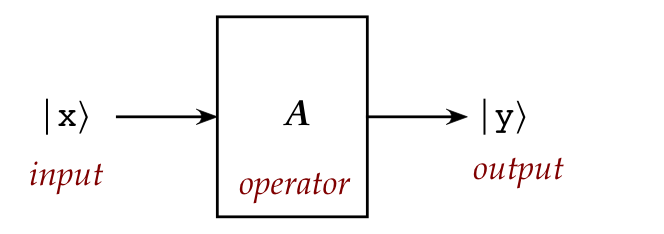
\includegraphics[width=4in]{notes/figs/n04/15operator.png}
        \caption{Input operator output}
        \label{fig:15operator.png}
    \end{figure}
    
    The idea of an operator can be extended to taking a function as input and producing a function as output shown in Figure \ref{fig:16operator2}.
    
    \begin{figure}
        \centering
        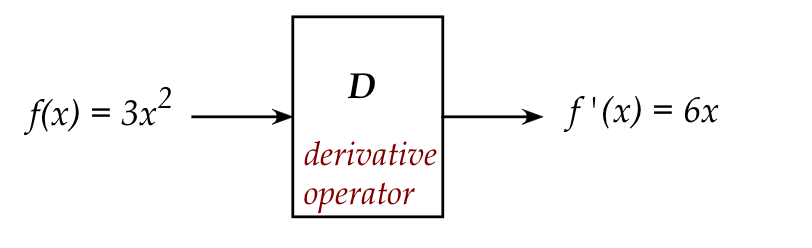
\includegraphics[width=4in]{notes/figs/n04/16operator2.png}
        \caption{Derivative operator}
        \label{fig:16operator2}
    \end{figure}
    
    In this case $D$ is the derivative operator so that $D f(x)=f^{\prime}(x)$. In quantum computing, all operators are matrices. Why then do we use the term operator? It's a good idea to use the more general term if you someday venture into quantum mechanics or more abstract linear algebra. Many papers and books use the term operator. Operators can be analyzed independent of whether they "act" on anything (vector or function). Operators can be combined. Example: A product of two matrix operators is a matrix operator. For the rest of the course, when you see operator, think matrix. The adjoint of a matrix operator: Recall: for any matrix $A$, its adjoint is the matrix $A^{\dagger}$. That is: $A^{\dagger}$ is the transpose and conjugate of $A$. Example: Let
    
    $$
    A=\left[\begin{array}{cc}
    1+i & -i \\
    i & 1+1
    \end{array}\right]
    $$
    
    Then the transpose is
    
    $$
    A^{T}=\left[\begin{array}{cc}
    1+i & i \\
    -i & 1+i
    \end{array}\right]
    $$
    
    And the conjugate of the transpose is:
    
    $$
    A^{\dagger}=\left(A^{T}\right)^{*}=\left[\begin{array}{cc}
    1-i & -i \\
    i & 1-i
    \end{array}\right]
    $$

    The two kinds of operators we're going to need are: Hermitian and unitary. Let's start with Hermitian: A Hermitian operator is an operator that satisfies $A=A^{\dagger}$. Thus for example
    
    $$
    A=\left[\begin{array}{cc}
    1 & -i \\
    i & 1
    \end{array}\right]
    $$
    
    is Hermitian. While
    
    $$
    B=\left[\begin{array}{cc}
    i & 1 \\
    1 & -i
    \end{array}\right]
    $$
    
    is not. Think of Hermitian as the complex generalization of a symmetric matrix for real numbers. A real matrix that's symmetric is Hermitian. A unitary operator: A unitary operator $A$ is one that satisfies $A^{\dagger} A=A A^{\dagger}=I$ That is, $A^{-1}=A^{\dagger}$. Examples: We saw that with
    
    $$
    H=\left[\begin{array}{rr}
    \frac{1}{\sqrt{2}} & \frac{1}{\sqrt{2}} \\
    \frac{1}{\sqrt{2}} & -\frac{1}{\sqrt{2}}
    \end{array}\right]
    $$
    
    $H^{\dagger} H=H H^{\dagger}=I$ and so $H$ is unitary. But
    
    $$
    A=\left[\begin{array}{cc}
    1 & -i \\
    i & 1
    \end{array}\right]
    $$
    
    is not. We're going to include a third type of operator that's closely related to Hermitian operators: projection. Recall that we used vectors to compute a projection matrix. In this spirit of "operator" terminology, we'll call this a projection operator or projector (as it's sometimes called). Recall that when $|u\rangle$ is projected on $|v\rangle$, the resulting vector (along $|v\rangle)$ is: $|v\rangle\langle v|| u\rangle$. We wrote the outerproduct $|v\rangle\langle v|$ earlier as the projector matrix
    
    $$
    P=|v\rangle\langle v|
    $$
    
    This is what we mean by the projector or projection operator. So far all we have are definitions of these three types of matrices, all of which play a crucial role in anything quantum-related. As a preview: We'll use unitary matrices to modify qubits. This will occur by the usual "matrix changes a vector by multiplication". Hermitian matrices are quite different: They will be used for something called measurement, a feature unique to quantum systems. And we won't be multiplying a vector by a Hermitian matrix. Instead, the matrix will be "applied" to a vector in a rather unusual way. Projector matrices play a role in the unusual application of Hermitian matrices, which is why the two kinds are intimately connected. Before we get to using these matrices, we'll need to understand some useful general properties.
    
    As a first step, let's point out something common to all three: All three matrices are square. Clearly, this is true for any projector: A projector is constructed from an outerproduct of an $n \times 1$ vector $|v\rangle$ and a $1 \times n$ vector $\langle v|$ : $(|v\rangle\langle v|)_{n \times n}$ Example:
    
    $$
    \left[\begin{array}{l}
    3 \\
    1 \\
    0
    \end{array}\right]\left[\begin{array}{lll}
    3 & 1 & 0
    \end{array}\right]=\left[\begin{array}{lll}
    9 & 3 & 0 \\
    3 & 1 & 0 \\
    0 & 0 & 0
    \end{array}\right]
    $$
    
    For a Hermitian operator, the squareness arises from requiring $A=A^{\dagger}$ : Suppose $A_{m \times n}$ has $m$ rows, $n$ columns. Because $A^{\dagger}$ is the conjugate transpose, $A^{\dagger}$ has $n$ rows, $m$ columns. The only way we can have $A=A^{\dagger}$ is if $m=n$. For unitary operator, the squareness comes from $A^{-1}=A^{\dagger}$ : We can of course compute $A^{\dagger}$ for a non-square matrix. But for this to equal the inverse, we must have $A A^{\dagger}=A^{\dagger} A=I$. Thus, for multiply compatibility on both sides, $A$ must be square. Because these are the key operators that motivate the theory, the term operator itself is defined to be "square". This makes sense for matrix operators. What about something like the differential operator? For more general operators, the generalization of "square" is the following: Consider a vector space $V$, a set of vectors closed under linear combinations $\Delta$ Any linear combination of vectors in $V$ will be in $V$. An operator is something that acts on a vector $v \in V$ to produce a vector in $V$. Sometimes this is expressed as: an operator is a mapping from a vector space to itself.

\subsection{Useful properties: adjoints and inner products}

    Note: For the most part, we will use "matrix proofs" because they are less abstract and amenable to examples. More abstract and generalized "slick" proofs do exist, which we'll use only occasionally. Where it makes sense, we'll accompany a proof with an example to illustrate the main ideas. More matrix notation: Sometimes we'll use $a_{i j}$ or $a_{i, j}$ to denote the element in row $i$ and column $j$ of a matrix $A$. The above introduces a new symbol, so one often uses $(A)_{i j}$ or $(A)_{i, j}$ directly. This has the advantage of conveniently describing the $i$-j-th element of a sum as in $(A+B)_{i j}$. Let's start with a really useful property when adjoints occur in an inner-product: Let's unpack the multiplication $A|x\rangle$ and write:
    
    $$
    A|x\rangle=\left[\begin{array}{ccc}
    a_{11} & \cdots & a_{1 n} \\
    \vdots & \vdots & \vdots \\
    a_{n 1} & \cdots & a_{n n}
    \end{array}\right]\left[\begin{array}{c}
    x_{1} \\
    \vdots \\
    x_{n}
    \end{array}\right]
    $$
    
    Then, taking the tranpose and conjugate of the result:
    
    $$
    (A|x\rangle)^{\dagger}=\left[\begin{array}{ccc}
    x_{1}^{*} & \cdots & x_{n}^{*}
    \end{array}\right]\left[\begin{array}{ccc}
    a_{11}^{*} & \cdots & a_{n 1}^{*} \\
    \vdots & \vdots & \vdots \\
    a_{1 n}^{*} & \cdots & a_{n n}^{*}
    \end{array}\right]=\langle x| A^{\dagger}
    $$
    
    Thus, although we're used to applying an operator from the left, one can apply from the right when it makes sense. Let's treat $A|x\rangle$ as the single vector $|A x\rangle$ and write
    
    $$
    \langle A x|=\left(\left[\begin{array}{ccc}
    a_{11} & \cdots & a_{1 n} \\
    \vdots & \vdots & \vdots \\
    a_{n 1} & \cdots & a_{n n}
    \end{array}\right]\left[\begin{array}{c}
    x_{1} \\
    \vdots \\
    x_{n}
    \end{array}\right]\right)^{\dagger}=\left[\begin{array}{lll}
    x_{1}^{*} & \cdots & x_{n}^{*}
    \end{array}\right]\left[\begin{array}{ccc}
    a_{11}^{*} & \cdots & a_{n 1}^{*} \\
    \vdots & \vdots & \vdots \\
    a_{1 n}^{*} & \cdots & a_{n n}^{*}
    \end{array}\right]=\langle x| A^{\dagger}
    $$
    
    Thus, we get the all important relation
    
    $$
    \langle A x|=\left\langle x\left|A^{\dagger}=\right| A x\right\rangle^{\dagger}
    $$
    
    Because of this,
    
    $$
    \left\langle A^{\dagger} x\right|=\langle x| A
    $$
    
    Now let's see how the same idea works with an inner-product. Suppose $|w\rangle$ is a vector and consider the inner-product $\langle w \mid A x\rangle$. Unpack this as
    
    $$
    \begin{aligned}
    \langle w \mid A x\rangle &=\left[\begin{array}{ccc}
    w_{1}^{*} & \cdots & w_{n}^{*}
    \end{array}\right]\left[\begin{array}{ccc}
    a_{11} & \cdots & a_{1 n} \\
    \vdots & \vdots & \vdots \\
    a_{n 1} & \cdots & a_{n n}
    \end{array}\right]\left[\begin{array}{r}
    x_{1} \\
    \vdots \\
    x_{n}
    \end{array}\right] \\
    =&\left(\left[\begin{array}{ccc}
    a_{11}^{*} & \cdots & a_{n 1}^{*} \\
    \vdots & \vdots & \vdots \\
    a_{1 n}^{*} & \cdots & a_{n n}^{*}
    \end{array}\right]\left[\begin{array}{r}
    w_{1} \\
    \vdots \\
    w_{n}
    \end{array}\right]\right)^{\dagger}\left[\begin{array}{r}
    x_{1} \\
    \vdots \\
    x_{n}
    \end{array}\right] \\
    =&\left\langle A^{\dagger} w \mid x\right\rangle
    \end{aligned}
    $$
    
    These properties are useful enough to memorialize as a formal result. Proposition 2.2: (Operator movement in inner-product) Let $A$ be an operator and $|x\rangle,|w\rangle$ be vectors. Then, i. $\langle A x|=\left\langle x\left|A^{\dagger}=\right| A x\right\rangle^{\dagger}$ ii. $\left\langle A^{\dagger} x\right|=\langle x| A$ iii. $\langle w \mid A x\rangle=\left\langle A^{\dagger} w \mid x\right\rangle$ iv. $\langle A w \mid x\rangle=\left\langle w \mid A^{\dagger} x\right\rangle$ The latter two are particularly useful, so let's put them in a diagram shown in Figure \ref{fig:17adjoint.png}.
    
    \begin{figure}
        \centering
        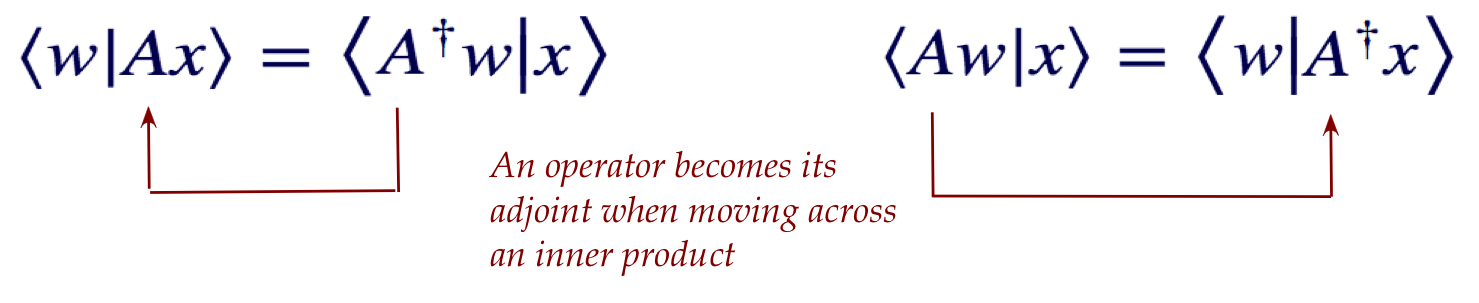
\includegraphics[width=4in]{notes/figs/n04/17adjoint.png}
        \caption{Operator becomes its adjoint when moving across an inner product}
        \label{fig:17adjoint.png}
    \end{figure}
    
    Recall: $A^{\prime}$ 's adjoint is $A^{\dagger}$, and $A^{\dagger \prime}$ s adjoint is $A$. Next, some basic properties of adjoints: Proposition 2.3: If $A$ and $B$ are operators and $\alpha$ is a complex number, then i. $\left(A^{\dagger}\right)^{\dagger}=A$ ii. $(\alpha A)^{\dagger}=\alpha^{*} A^{\dagger}$ iii. $(A+B)^{\dagger}=A^{\dagger}+B^{\dagger}$ iv. $(A B)^{\dagger}=B^{\dagger} A^{\dagger}$. Proof: For any matrix $A$, let $(A)_{i j}$ represent the element in row $i$ and column $\mathrm{j}$. i. Observe that $(A)_{i j}$, the i-j-th element of $A$ becomes $(A)_{j i}^{*}$ in $A^{\dagger}$. Thus, applying conjugate transpose again results in $(A)_{i j}$. ii. $(\alpha A)$ multiplies each element of $A$ by $\alpha$. Thus, the i-j-th element of $(\alpha A)^{\dagger}$

    $$
    \begin{aligned}
    \left((\alpha A)^{\dagger}\right)_{i j} &=\left((\alpha A)_{j i}\right)^{*} & & \text { Transpose first } \\
    &=\left(\alpha(A)_{j i}\right)^{*} & & \text { Pull out } \alpha \\
    &=\alpha^{*}(A)_{j i}^{*} & & \text { a gets conjugated outside } \\
    &=\alpha^{*}\left(A^{\dagger}\right)_{i j} & & \text { By definition of conjugate transpose }
    \end{aligned}
    $$
    
    iii. Again, we examine how the $\mathrm{i}-\mathrm{j}$-th element of $(A+B)^{\dagger}$ comes about:
    
    $$
    \begin{aligned}
    \left((A+B)^{\dagger}\right)_{i j} &=\left((A+B)^{*}\right)_{j i} & & \text { Conjugate first, then transpose } \\
    &=\left(A^{*}+B^{*}\right)_{j i} & & \text { Conjugate distributes over }+\\
    &=\left(A^{*}\right)_{j i}+\left(B^{*}\right)_{j i} & & \text { Matrix addiition } \\
    &=\left(A^{\dagger}\right)_{i j}+\left(B^{\dagger}\right)_{i j} & & \text { Conjugate trunspose }
    \end{aligned}
    $$
    
    iv. Now for $(A B)^{\dagger}=B^{\dagger} A^{\dagger}$. Unfortunately, getting at the $i$-j-th element of $A B$ is messy because it is computed with row i of $A$ and column $j$ of $B$. Instead, we'll demonstrate a rather slick proof using inner-products:
    
    $$
    \begin{aligned}
    \left\langle w \mid(A B)^{\dagger} x\right\rangle &=\langle(A B) w \mid x\rangle & & \text { Operator movement in inner-prodi } \\
    &=\langle A(B w) \mid x\rangle & & \text { Associativity } \\
    &=\left\langle B w \mid A^{\dagger} x\right\rangle & & \text { Operator movement in reverse } \\
    &=\left\langle w \mid B^{\dagger}\left(A^{\dagger} x\right)\right\rangle & & \text { Operator movement again } \\
    &=\left\langle w \mid\left(B^{\dagger} A^{\dagger}\right) x\right\rangle & & \text { Associativity }
    \end{aligned}
    $$
    
    Since this is true for all vectors $|w\rangle,|x\rangle,(A B)^{\dagger}=B^{\dagger} A^{\dagger}$.

\subsection{Useful properties: Hermitian operators}

    Recall the definition of a Hermitian operator: An operator $A$ is Hermitian if $A^{\dagger}=A$. Now let's run through some properties: Proposition 2.4: Let $A, B$ be Hermitian operators. Then i. $A+B$ is Hermitian ii. $\alpha A$ is Hermitian for real numbers $\alpha$. Proof: For the first part
    
    $$
    \begin{aligned}
    (A+B)_{i j}^{\dagger} &=(A+B)_{j i}^{*} & & \text { Conjugate, then transpose } \\
    &=\left(A^{*}+B^{*}\right)_{j i} & & \text { Conjugate distributes } \\
    &=A_{j i}^{*}+B_{j i}^{*} & & \text { Matrix addition } \\
    &=A_{i j}^{\dagger}+B_{i j}^{\dagger} & & \text { Definition of conjugate-transpose } \\
    &=A_{i j}+B_{i j} & & \text { A, B are Hermitian } \\
    &=(A+B)_{i j} & &
    \end{aligned}
    $$
    
    For the second
    
    $$
    (\alpha A)_{i j}^{\dagger}=(\alpha A)_{j i}^{*}=\left(\alpha^{*} A^{*}\right)_{j i}=\alpha A_{j i}^{*}=\alpha A_{j i}^{\dagger}=\alpha A_{i j}=(\alpha A)_{i j}
    $$
    
    Recall the definition of a Hermitian operator: An operator $A$ is Hermitian if $A^{\dagger}=A$.
    Now let's run through some properties: Proposition 2.4: Let $A, B$ be Hermitian operators. Then i. $A+B$ is Hermitian ii. $\alpha A$ is Hermitian for real numbers $\alpha$. Proof: For the first part
    
    $$
    \begin{aligned}
    (A+B)_{i j}^{\dagger} &=(A+B)_{j i}^{*} & & \text { Conjugate, then transpose } \\
    &=\left(A^{*}+B^{*}\right)_{j i} & & \text { Conjugate distributes } \\
    &=A_{j i}^{*}+B_{j i}^{*} & & \text { Matrix addition } \\
    &=A_{i j}^{\dagger}+B_{i j}^{\dagger} & & \text { Definition of conjugate-transpose } \\
    &=A_{i j}+B_{i j} & & \text { A, B are Hermitian } \\
    &=(A+B)_{i j} & &
    \end{aligned}
    $$
    
    For the second
    
    $$
    (\alpha A)_{i j}^{\dagger}=(\alpha A)_{j i}^{*}=\left(\alpha^{*} A^{*}\right)_{j i}=\alpha A_{j i}^{*}=\alpha A_{j i}^{\dagger}=\alpha A_{i j}=(\alpha A)_{i j}
    $$

    Proposition 2.5: The diagonal elements of a Hermitian matrix are real numbers. Proof: Example: Consider
    
    $$
    A=\left[\begin{array}{ccc}
    \ddots & \ldots & \\
    \vdots & a+i b & \vdots \\
    & \ldots & \ddots
    \end{array}\right]
    $$
    
    and let's focus on one of the diagonal elements shown. Then the transpose conjugate will end up conjugating this element
    
    $$
    A^{\dagger}=\left[\begin{array}{ccc}
    \ddots & \cdots & \\
    \vdots & a-i b & \vdots \\
    & \cdots & \ddots
    \end{array}\right]
    $$
    
    Thus, $A^{\dagger}=A$ implies $a+i b=a-i b$ or $b=0$. Proposition 2.6: The eigenvalues of a Hermitian operator are real. Proof: Suppose the Hermitian operator $A$ has eigenvalue $\lambda$ for eigenvector $v$, i.e. $A|v\rangle=\lambda|v\rangle$. Recall from earlier, for any operator $A$ and vectors $|w\rangle,|x\rangle$
    
    $$
    \langle w \mid A x\rangle=\left\langle A^{\dagger} w \mid x\right\rangle
    $$
    
    For a Hermitian operator
    
    $$
    \langle w \mid A x\rangle=\langle A w \mid x\rangle
    $$
    
    Next, substitute $w=v, x=v$ to get
    
    $$
    \langle A v \mid v\rangle=\langle v \mid A v\rangle
    $$
    
    Applying the eigenvalue relation on both sides,
    
    $$
    \langle\lambda v \mid v\rangle=\langle v \mid \lambda v\rangle
    $$
    
    and factoring out $\lambda$,
    
    $$
    \lambda^{*}\langle v \mid v\rangle=\lambda\langle v \mid v\rangle
    $$
    
    Thus, $\lambda^{*}=\lambda$ which makes it real. Application: This turns out to matter when a Hermitian matrix is written in its eigenbasis, in which case the only non-zero elements (the eigenvalues) are on the diagonal. These eigenvalues correspond to real-world quantities that are observed (such as energy, for example). Proposition 2.7: Eigenvectors corresponding two distinct eigenvalues of a Hermitian operator are orthogonal. Proof: Let $\lambda_{1}, \lambda_{2}$ be two distinct eigenvalues corresponding to eigenvectors $\left|v_{1}\right\rangle,\left|v_{2}\right\rangle$. Then
    
    $$
    \left\langle A v_{1} \mid v_{2}\right\rangle=\left\langle\lambda_{1} v_{1} \mid v_{2}\right\rangle=\lambda_{1}^{*}\left\langle v_{1} \mid v_{2}\right\rangle=\lambda_{1}\left\langle v_{1} \mid v_{2}\right\rangle
    $$
    
    (The last step because eigenvalues are real.) Next,
    
    $$
    \left\langle v_{1} \mid A v_{2}\right\rangle=\left\langle v_{1} \mid \lambda_{2} v_{2}\right\rangle=\lambda_{2}\left\langle v_{1} \mid v_{2}\right\rangle
    $$
    
    These two must be equal because
    
    $$
    \left\langle A v_{1} \mid v_{2}\right\rangle=\left\langle v_{1} \mid A^{\dagger} v_{2}\right\rangle=\left\langle v_{1} \mid A v_{2}\right\rangle
    $$
    
    since $A=A^{\dagger}$. Thus, subtracting
    
    $$
    \left(\lambda_{1}-\lambda_{2}\right)\left\langle v_{1} \mid v_{2}\right\rangle=0
    $$
    
    Which means $\left\langle v_{1} \mid v_{2}\right\rangle=0$ since the eigenvalues are assumed to be distinct. Application: In quantum computing, we will exploit this to reason about Hermitians. Proposition 2.8: (The spectral theorem for Hermitian operators) A Hermitian operator $A$ on an n-dimensional vector space $V$ has $n$ orthonormal eigenvectors $\left|v_{1}\right\rangle, \ldots,\left|v_{n}\right\rangle$ with eigenvalues $\lambda_{1}, \ldots, \lambda_{n}$ such that: i. $\left|v_{1}\right\rangle, \ldots,\left|v_{n}\right\rangle$ form a basis for $V$. ii. $A$ is a diagonal matrix
    
    $$
    \left[\begin{array}{cccc}
    \lambda_{1} & 0 & 0 & 0 \\
    0 & \lambda_{2} & 0 & 0 \\
    \vdots & 0 & \ddots & 0 \\
    0 & 0 & 0 & \lambda_{n}
    \end{array}\right]
    $$
    
    when written in the basis $\left|v_{1}\right\rangle, \ldots,\left|v_{n}\right\rangle$.
    
    $$
    \text { iii. } A=\sum_{i=1}^{n} \lambda_{i}\left|v_{i}\right\rangle\left\langle v_{i}\right| \text {. }
    $$
    
    Proof: The proof is somewhat long and uses induction; we'll refer you to Axler's book.
    
\subsection{Useful properties: orthonormality and projector operators}

    Squared amplitudes add up to 1 : Proposition 2.9: Let $\alpha_{i}$ 's be the amplitudes (coefficients) when $|u\rangle=\sum_{i} \alpha_{i}\left|v_{i}\right\rangle$ is expressed in the (orthonormal) basis $\left|v_{1}\right\rangle, \ldots,\left|v_{n}\right\rangle$. Then
    
    $$
    \sum_{i}\left|\alpha_{i}\right|^{2}=1
    $$
    
    Proof: Algebra
    
    $=1$
    
    Application: As we'll see in the next module, this is fundamental to the theory when the $\left|\alpha_{i}\right|^{2}$ 's are interpreted as probabilities. A full set of probabilities, as we know, must sum to 1 . Projectors and Hermitians: Proposition 2.10: A projector is idempotent. That is,
    
    $$
    P_{v}^{2}=P_{v}
    $$
    
    so that when a projector is applied twice in succession the same result obtains. Proof:
    
    $$
    P_{v}^{2}=P_{v} P_{v}=|v\rangle\langle v|| v\rangle\langle v|=| v\rangle(\langle v \mid v\rangle)\langle v|=| v\rangle \times 1 \times\langle v|=| v\rangle\langle v|=P_{v}
    $$
    
    Application: this matches intuition. When we project a vector $|u\rangle$ onto $|v\rangle$, we get a vector along $|v\rangle$. Suppose we call that vector $|y\rangle=P_{v}|u\rangle$. Applying $P_{v}$ twice is the same as applying $P_{v}$ to $|y\rangle$, i.e., $P_{v} P_{v}|u\rangle=P_{v}|y\rangle$. But the projection of a vector that's already along $|v\rangle$ leaves the vector unchanged. Thus, $P_{v}|y\rangle=|y\rangle$. Which means $P_{v} P_{v}|u\rangle=P_{v}|u\rangle$ or $P_{v}^{2}=P_{v}$. Proposition 2.11: A projector is Hermitian. That is, the projector $P_{v}=|v\rangle\langle v|$ satisfies $P^{\dagger}=P$. Proof: See earlier exercise. Application: We will see a stronger result below, but we'll need this one when projectors need to be combined for multiple qubits. Proposition 2.12: The projector $P_{v}=|v\rangle\langle v|$ has eigenvector $|v\rangle$ with eigenvalue 1. Proof: Clearly 
    
    $$ 
    P_{v}|v\rangle=|v\rangle\langle v|| v\rangle=|v\rangle\langle v \mid v\rangle=|v\rangle
    $$
    Proposition 2.13: For real number $\lambda$ and projector $P_{v}=|v\rangle\langle v|$, the operator $\lambda P_{v}$ is Hermitian with eigenvector $|v\rangle$ and eigenvalue $\lambda$. Proof: The fact that $\lambda P_{v}$ is Hermitian follows from the proposition earlier that showed that for any real scalar $\lambda$ and Hermitian $A$, the operator $\lambda A$ is Hermitian. Next,
    
    $$
    \left(\lambda P_{v}\right)|v\rangle=\lambda P_{v}|v\rangle=\lambda|v\rangle
    $$
    
    Which makes $|v\rangle$ an eigenvector of $\lambda P_{v}$ with eigenvalue $\lambda$. Proposition 2.14: Let $P_{v_{1}}, \ldots, P_{v_{n}}$ be projectors for basis vectors $\left|v_{1}\right\rangle, \ldots,\left|v_{n}\right\rangle$. Next, let $\lambda_{1}, \ldots, \lambda_{n}$ be real numbers. Then the real linear combination
    
    $$
    A=\sum_{i} \lambda_{i} P_{v_{i}}=\sum_{i} \lambda_{i}\left|v_{i}\right\rangle\left\langle v_{i}\right|
    $$
    
    is a Hermitian operator with eigenvectors $\left|v_{1}\right\rangle, \ldots,\left|v_{n}\right\rangle$ and corresponding eigenvalues $\lambda_{1}, \ldots, \lambda_{n}$. Proof: The previous proposition shows that each $\lambda_{i} P_{v_{i}}$ is Hermitian. The sum of Hermitians is Hermitian. Next,
    
    $$
    A\left|v_{i}\right\rangle=\left(\sum_{k} \lambda_{k} P_{v_{k}}\right)\left|v_{i}\right\rangle=\lambda_{i} P_{v_{i}}\left|v_{i}\right\rangle=\lambda_{i}\left|v_{i}\right\rangle
    $$
    
    Application: What we've shown is that some Hermitians have the particular linear-combination-of-projectors structure as above. These, in fact, will be the only type of Hermitians we'll encounter in quantum computing. And this structure is the key to understanding one of the most counter-intuitive aspects of quantum computing: measurement.

\subsection{Useful properties: unitary operators}

    Recall: A unitary operator $A$ is one that satisfies $A^{\dagger} A=A A^{\dagger}=I$. That is, $A^{-1}=A^{\dagger}$. Let's work through some useful properties of unitary operators Proposition 2.15: A unitary operator preserves inner-products: $\langle A u \mid A v\rangle=\langle u \mid v\rangle$. Proof: We'll exploit the operator-across-inner-product property here:
    
    $$
    \langle A u \mid A v\rangle=\left\langle A^{\dagger}(A u) \mid v\right\rangle=\left\langle\left(A^{\dagger} A\right) u\right)|v\rangle=\langle I u \mid v\rangle=\langle u \mid v\rangle
    $$
    
    Proposition 2.16: A unitary operator preserves lengths: $|A u|=|u|$. Proof: From the above property
    
    $$
    |A u|^{2}=\langle A u \mid A u\rangle=\langle u \mid u\rangle=|u|^{2}
    $$
    
    Proposition 2.17: If $A$ is unitary so are $A^{\dagger}$ and $A^{-1}$. Proof: The definition of unitary is symmetric: $A$ is unitary if $A A^{\dagger}=A^{\dagger} A=I$. Thus, $A^{\dagger}$ is also unitary, and because $A^{-1}=A^{\dagger}$, it too is unitary. Proposition 2.18: The columns of $A$ are orthonormal, as are the rows. Proof: Consider the product $A^{\dagger} A=I$ and the i-j-th element of $I$. This is formed by multiplying the i-th row of $A^{\dagger}$ (conjugate of the $\mathrm{i}$-th column) into the j-th column of $A$. When $i \neq j$ we get 0 , meaning the $i$ and $j$ columns are orthogonal. Similarly, when $i=j$, we get a diagonal element of $I$, which is 1 , meaning each column is of unit length. The argument for orthonormality of the rows uses the same arguments with $A A^{\dagger}=I$. Proposition 2.19: If $\left|v_{1}\right\rangle, \ldots,\left|v_{n}\right\rangle$ are orthonormal, so are $\left|A v_{1}\right\rangle, \ldots,\left|A v_{n}\right\rangle$ when $A$ is unitary. Proof: What we need to show is that $\left\langle A v_{i} \mid A v_{j}\right\rangle=0$ if $i \neq j$ and $\left\langle A v_{i} \mid A v_{j}\right\rangle=1$ if $i=j$. This follows from the preservation of inner products: $\left\langle A v_{i} \mid A v_{j}\right\rangle=\left\langle v_{i} \mid v_{j}\right\rangle$. Proposition 2.20: If $A, B$ are unitary, then so are $A B$ and $B A$. Proof:
    
    $$
    (A B)^{\dagger}(A B)=\left(B^{\dagger} A^{\dagger}\right)(A B)=B^{\dagger}\left(A^{\dagger} A\right) B=B^{\dagger}(I) B=B^{\dagger} B=I
    $$
    
    The proof for $B A$ is similar. Application: The product rule above is probably the most frequently applied. Think of $A$ and $B$ as two gates that occur in sequence. The net result is the product, as we will see. The other properties above are useful in reasoning about unitary matrices and building the theory.

\subsection{The operator sandwich}

    Let's now return to applying an operator from the left, and from the right: We have seen that
    
    $$
    A|v\rangle=|A v\rangle
    $$
    
    and thus there is no ambiguity in writing either way. Similarly, when applying from the right:
    
    $$
    \langle A u|=\langle u| A^{\dagger}
    $$
    
    which means
    
    $$
    \left\langle A^{\dagger} u\right|=\langle u| A
    $$
    
    Next, consider the expression
    
    $\langle u|A| v\rangle$
    
    If $A$ were applied to the left of $|v\rangle$, this would become:
    
    $$
    \langle u|A| v\rangle=\langle u \mid A v\rangle
    $$
    
    If $A$ were applied to the right of $\langle u|$ :
    
    $$
    \langle u|A| v\rangle=\left\langle A^{\dagger} u \mid v\right\rangle
    $$
    
    But both result in the same inner product:
    
    $$
    \langle u \mid A v\rangle=\left\langle A^{\dagger} u \mid v\right\rangle
    $$
    
    Thus, the actual calculation could be done either way. We will use the so-called operator sandwich to write this as $\langle u|A| v\rangle$ where it's implied that we have two ways of performing the calculation. Note: $\langle u|A| v\rangle$ is still an inner-product, and will result in a number. This result applies to any operator, not just Hermitian and unitary operators.
    Let's see how this works through an example: Suppose
    
    $$
    A=\left[\begin{array}{cc}
    i & 1 \\
    1 & -i
    \end{array}\right]
    $$
    
    $$
    |u\rangle=\left[\begin{array}{l}
    1 \\
    0
    \end{array}\right]
    $$
    
    $$
    |v\rangle=\left[\begin{array}{c}
    \frac{1}{\sqrt{2}} \\
    \frac{1}{\sqrt{2}}
    \end{array}\right]
    $$
    
    We'll first calculate
    
    $$
    \begin{aligned}
    \langle u|A| v\rangle &=\langle u \mid A v\rangle \\
    &=\left[\begin{array}{ll}
    1 & 0
    \end{array}\right]\left(\left[\begin{array}{cc}
    i & 1 \\
    1 & -i
    \end{array}\right]\left[\begin{array}{c}
    \frac{1}{\sqrt{2}} \\
    \frac{1}{\sqrt{2}}
    \end{array}\right]\right) \\
    &=\left[\begin{array}{ll}
    1 & 0
    \end{array}\right]\left[\begin{array}{c}
    \frac{1+i}{\sqrt{2}} \\
    \frac{1-i}{\sqrt{2}}
    \end{array}\right] \\
    &=\frac{1+i}{\sqrt{2}}
    \end{aligned}
    $$
    
    $$
    =\left[\begin{array}{ll}
    1 & 0
    \end{array}\right]\left[\begin{array}{c}
    \frac{1+i}{\sqrt{2}} \\
    \frac{1-i}{\sqrt{2}}
    \end{array}\right]
    $$
    
    $$
    =\frac{1+i}{\sqrt{2}}
    $$
    
    And now the other way:
    
    $$
    \langle u|A| v\rangle=\left\langle A^{\dagger} u \mid v\right\rangle
    $$
    
    First, note that

    $$
    A^{\dagger} u=\left[\begin{array}{cc}
    -i & 1 \\
    1 & i
    \end{array}\right]\left[\begin{array}{l}
    1 \\
    0
    \end{array}\right]=\left[\begin{array}{r}
    -i \\
    1
    \end{array}\right]
    $$
    
    The inner-product of the conjugated row $\left\langle A^{\dagger} u\right|$ with $|v\rangle$ then is
    
    $$
    \left\langle A^{\dagger} u \mid v\right\rangle=\left[\begin{array}{ll}
    i & 1
    \end{array}\right]\left[\begin{array}{c}
    \frac{1}{\sqrt{2}} \\
    \frac{1}{\sqrt{2}}
    \end{array}\right]=\frac{1+i}{\sqrt{2}}
    $$
    
    Which is, as expected, the same result (number) as before. How it's used: The operator sandwich is used frequently and is yet another notational and conceptual idea we need to get comfortable with. Here's one example with a projector: Consider the projection of $|u\rangle$ on $|v\rangle$. We know that the projector is written as the outer-product
    
    $$
    P_{v}=|v\rangle\langle v|
    $$
    
    Now consider the sandwich
    
    $$
    \left\langle u\left|P_{v}\right| u\right\rangle=\langle u|| v\rangle\langle v|| u\rangle=\langle u \mid v\rangle\langle v \mid u\rangle=(\langle v \mid u\rangle)^{*}\langle v \mid u\rangle=|\langle v \mid u\rangle|^{2}
    $$
    
    Thus, $\left\langle u\left|P_{v}\right| u\right\rangle$ is the squared magnitude of the coefficient in the projection. Here's another example with projectors: The projected vector when projecting $|u\rangle$ along $|v\rangle$ is: $P_{v}|u\rangle$. Suppose we want the length of this vector: $\left.\left|P_{v}\right| u\right\rangle \mid$. We can write the squared magnitude as: 
    
    $$
    \begin{aligned}
    \left.\left|P_{v}\right| u\right\rangle\left.\right|^{2} &=\left(P_{v}|u\rangle\right)^{\dagger} P_{v}|u\rangle & & \text { Inner product of } P_{v}|u\rangle \text { with itself } \\
    &=\left(\langle u| P_{v}^{\dagger}\right) P_{v}|u\rangle & & \text { Apply adjoint } \\
    &=\left\langle u\left|P_{v} P_{v}\right| u\right\rangle & & \text { A projector is Hermitian } \\
    &=\left\langle u\left|P_{v}\right| u\right\rangle & & \text { A projector is idempotent }
    \end{aligned}
    $$
    
    Next,
    
    $$
    \begin{aligned}
    \left\langle u\left|P_{v_{1}}\right| u\right\rangle &=\left\langle\alpha v_{1}+\beta v_{2}|\alpha| v_{1}\right\rangle & & \text { Sub for }|u\rangle \text { on left, and above-computed } P_{v 1}|u\rangle \\
    &=\alpha\left\langle\alpha v_{1}+\beta v_{2} \mid v_{1}\right\rangle & & \text { Move second } \alpha \\
    &=\alpha\left(\alpha^{*}\left\langle v_{1} \mid v_{1}\right\rangle+\beta^{*}\left\langle v_{2} \mid v_{1}\right\rangle\right) & & \text { Left-side linearity } \\
    &=\alpha \alpha^{*} & & \text { Basis vector inner-products } \\
    &     =|\alpha|^{2} & &
    \end{aligned}
    $$

\subsection{A key question: what is the basis of the moment?}

    In the regular linear algebra we've studied: We see multiple bases but we typically only use coordinates from the standard basis. We rarely if ever switch coordinates to a non-standard basis. And almost never express a matrix in a non-standard basis. In quantum computing (and mechanics), on the other hand: We use different bases at different times. It is essential to know at any time which basis is being used, and for what. When using a non-standard basis we have two options: 1. Use the non-standard basis but using coordinates from the standard basis for calculations. 2. Convert to the coordinates of the non-standard basis and then calculate from there. We'll illustrate both below. Let's work through an example to clarify using Figure \ref{fig:18basischange.png}.
    
    \begin{figure}
        \centering
        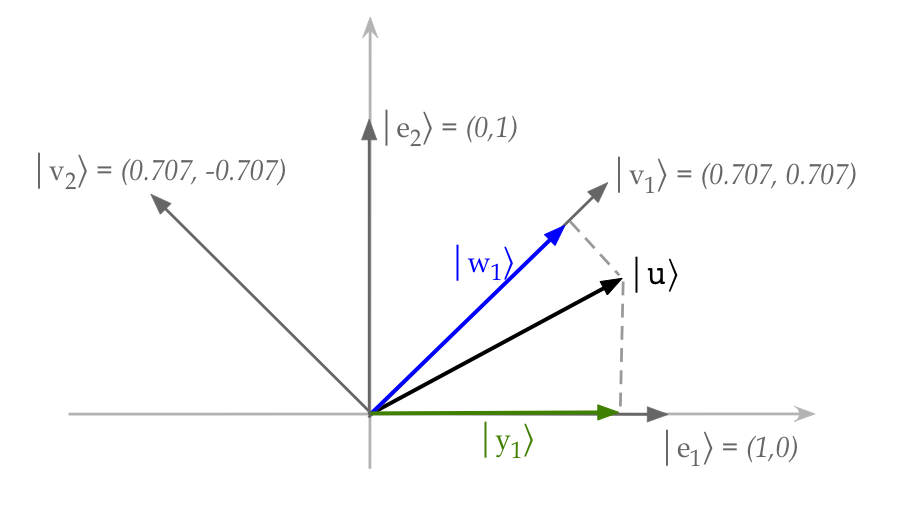
\includegraphics[width=4in]{notes/figs/n04/18basischange.png}
        \caption{Real Number Vectors}
        \label{fig:18basischange.png}
    \end{figure}
    
    We'll use real numbers so that we can draw vectors (above). Here, there are two bases shown: The standard basis:
    
    $$
    \left|e_{1}\right\rangle=\left[\begin{array}{l}
    1 \\
    0
    \end{array}\right] \quad\left|e_{2}\right\rangle=\left[\begin{array}{l}
    0 \\
    1
    \end{array}\right]
    $$
    
    Another basis (called the Hadamard basis):
    
    $$
    \left|v_{1}\right\rangle=\left[\begin{array}{c}
    \frac{1}{\sqrt{2}} \\
    \frac{1}{\sqrt{2}}
    \end{array}\right] \quad\left|v_{2}\right\rangle=\left[\begin{array}{c}
    \frac{1}{\sqrt{2}} \\
    -\frac{1}{\sqrt{2}}
    \end{array}\right]
    $$
    
    Because $\frac{1}{\sqrt{2}} \approx 0.707$, the coordinates are labeled as such. Notice that the diagram shows projections of the vector
    
    $$
    |u\rangle=\left[\begin{array}{c}
    \frac{\sqrt{3}}{2} \\
    \frac{1}{2}
    \end{array}\right]
    $$
    
    along $\left|e_{1}\right\rangle$ (in green) and along $\left|v_{1}\right\rangle$ (in blue). Let $\left|y_{1}\right\rangle \triangleq$ projection along $\left|e_{1}\right\rangle$, $\left|w_{1}\right\rangle \triangleq$ projection along $\left|v_{1}\right\rangle$, Let's first use standard-basis coordinates for calculations: The projector for $\left|e_{1}\right\rangle$ is:
    
    $$
    P_{e_{1}}=\left|e_{1}\right\rangle\left\langle e_{1}\right|=\left[\begin{array}{l}
    1 \\
    0
    \end{array}\right]\left[\begin{array}{ll}
    1 & 0
    \end{array}\right]=\left[\begin{array}{ll}
    1 & 0 \\
    0 & 0
    \end{array}\right]
    $$
    
    Then, the projection of $|u\rangle$ along $\left|e_{1}\right\rangle$ is:
    
    $$
    \left|y_{1}\right\rangle=P_{e_{1}}|u\rangle=\left[\begin{array}{ll}
    1 & 0 \\
    0 & 0
    \end{array}\right]\left[\begin{array}{c}
    \frac{\sqrt{3}}{2} \\
    \frac{1}{2}
    \end{array}\right]=\left[\begin{array}{c}
    \frac{\sqrt{3}}{2} \\
    0
    \end{array}\right]
    $$
    
    The projector for $\left|v_{1}\right\rangle$ is:
    
    $$
    P_{v_{1}}=\left|v_{1}\right\rangle\left\langle v_{1}\right|=\left[\begin{array}{c}
    \frac{1}{\sqrt{2}} \\
    \frac{1}{\sqrt{2}}
    \end{array}\right]\left[\begin{array}{ll}
    \frac{1}{\sqrt{2}} & \frac{1}{\sqrt{2}}
    \end{array}\right]=\left[\begin{array}{ll}
    \frac{1}{2} & \frac{1}{2} \\
    \frac{1}{2} & \frac{1}{2}
    \end{array}\right]
    $$
    
    And therefore the projection of $|u\rangle$ along $\left|v_{1}\right\rangle$ is:
    
    $$
    \left|w_{1}\right\rangle=P_{v_{1}}|u\rangle=\left[\begin{array}{cc}
    \frac{1}{2} & \frac{1}{2} \\
    \frac{1}{2} & \frac{1}{2}
    \end{array}\right]\left[\begin{array}{c}
    \frac{\sqrt{3}}{2} \\
    \frac{1}{2}
    \end{array}\right]=\left[\begin{array}{c}
    \frac{\sqrt{3}+1}{2} \\
    \frac{\sqrt{3}+1}{2}
    \end{array}\right]
    $$
    
    This should make sense because $\left|v_{1}\right\rangle$ is at a $45^{\circ}$ angle and so both coordinates should be the same. Let's point out: $\circ$ Although $\left|v_{1}\right\rangle,\left|v_{2}\right\rangle$ is a different basis than $\left|e_{1}\right\rangle,\left|e_{2}\right\rangle$, all calculations have been done using coordinates from $\left|e_{1}\right\rangle,\left|e_{2}\right\rangle$ (standard-basis). We know this because $\left|v_{1}\right\rangle,\left|v_{2}\right\rangle$ themselves were written in standard-basis coordinates:
    
    $$
    \left|v_{1}\right\rangle=\left[\begin{array}{c}
    \frac{1}{\sqrt{2}} \\
    \frac{1}{\sqrt{2}}
    \end{array}\right] \quad\left|v_{2}\right\rangle=\left[\begin{array}{r}
    \frac{1}{\sqrt{2}} \\
    -\frac{1}{\sqrt{2}}
    \end{array}\right]
    $$
    
    Thus, all the calculations have been done in the standard basis.
    
    Now let's see what it's like to perform calculations in the other basis, the $\left|v_{1}\right\rangle,\left|v_{2}\right\rangle$ basis: First, we'll ask: what are the coordinates of the basis vectors $\left|v_{1}\right\rangle,\left|v_{2}\right\rangle$ in their own basis? To get the coordinates of $\left|v_{1}\right\rangle$ in the $\left|v_{1}\right\rangle,\left|v_{2}\right\rangle$ basis, we need to solve
    
    $$
    \alpha_{1}\left|v_{1}\right\rangle+\alpha_{2}\left|v_{2}\right\rangle=\left|v_{1}\right\rangle
    $$
    
    That is, what linear combination of the basis vectors gives us the target vector $\left|v_{1}\right\rangle$, in this case)? Clearly, the solution is $\alpha_{1}=1, \alpha_{2}=0$. Similarly, to get the coordinates of $\left|v_{2}\right\rangle$, we solve
    
    $$
    \beta_{1}\left|v_{1}\right\rangle+\beta_{2}\left|v_{2}\right\rangle=\left|v_{2}\right\rangle
    $$
    
    to get $\beta_{1}=0, \beta_{2}=1$. Thus the coordinates of $\left|v_{1}\right\rangle,\left|v_{2}\right\rangle$ in the new basis are:
    
    $$
    \left|v_{1}\right\rangle=\left[\begin{array}{l}
    1 \\
    0
    \end{array}\right] \quad\left|v_{2}\right\rangle=\left[\begin{array}{l}
    0 \\
    1
    \end{array}\right]
    $$
    
    Surprised by this (simple) result? We'll have more to say about this below. Next, let's write $|u\rangle$ in the $\left|v_{1}\right\rangle,\left|v_{2}\right\rangle$ basis: We need to solve
    
    $$
    \gamma_{1}\left|v_{1}\right\rangle+\gamma_{2}\left|v_{2}\right\rangle=|u\rangle
    $$
    
    How do we solve for $\gamma_{1}, \gamma_{2}$ without knowing $|u\rangle$? The key insight is that $\gamma_{1}, \gamma_{2}$ will be the same no matter which basis is used. So, since we know $|u\rangle$ in the standard basis, we'll first use the standard basis: That is,
    
    $$
    \gamma_{1}\left[\begin{array}{c}
    \frac{1}{\sqrt{2}} \\
    \frac{1}{\sqrt{2}}
    \end{array}\right]+\gamma_{2}\left[\begin{array}{r}
    \frac{1}{\sqrt{2}} \\
    -\frac{1}{\sqrt{2}}
    \end{array}\right]=\left[\begin{array}{c}
    \frac{\sqrt{3}}{2} \\
    \frac{1}{2}
    \end{array}\right]
    $$
    
    Which we can write in matrix form:
    
    $$
    \left[\begin{array}{cc}
    \frac{1}{\sqrt{2}} & \frac{1}{\sqrt{2}} \\
    \frac{1}{\sqrt{2}} & -\frac{1}{\sqrt{2}}
    \end{array}\right]\left[\begin{array}{l}
    \gamma_{1} \\
    \gamma_{2}
    \end{array}\right]=\left[\begin{array}{c}
    \frac{\sqrt{3}}{2} \\
    \frac{1}{2}
    \end{array}\right]
    $$
    
    We could solve this the usual linear-equation way, but notice that the matrix is unitary, which means the inverse is the adjoint. Thus
    
    $$
    |u\rangle=\left[\begin{array}{cc}
    \frac{1}{\sqrt{2}} & \frac{1}{\sqrt{2}} \\
    \frac{1}{\sqrt{2}} & -\frac{1}{\sqrt{2}}
    \end{array}\right]\left[\begin{array}{c}
    \frac{\sqrt{3}}{2} \\
    \frac{1}{2}
    \end{array}\right]=\left[\begin{array}{c}
    \frac{\sqrt{3}+1}{2 \sqrt{2}} \\
    \frac{\sqrt{3}-1}{2 \sqrt{2}}
    \end{array}\right]
    $$
    
    Now that we know the coordinates of $|u\rangle$ in the new basis, let's compute the projection along $\left|v_{1}\right\rangle$: The projector in new coordinates is:
    
    $$
    P_{v_{1}}=\left|v_{1}\right\rangle\left\langle v_{1}\right|=\left[\begin{array}{l}
    1 \\
    0
    \end{array}\right]\left[\begin{array}{ll}
    1 & 0
    \end{array}\right]=\left[\begin{array}{ll}
    1 & 0 \\
    0 & 0
    \end{array}\right]
    $$
    
    Applying this to $|u\rangle$:
    
    $$
    P_{v_{1}}|u\rangle=\left[\begin{array}{ll}
    1 & 0 \\
    0 & 0
    \end{array}\right]\left[\begin{array}{c}
    \frac{\sqrt{3}+1}{2 \sqrt{2}} \\
    \frac{\sqrt{3}-1}{2 \sqrt{2}}
    \end{array}\right]=\left[\begin{array}{c}
    \frac{\sqrt{3}+1}{2 \sqrt{2}} \\
    0
    \end{array}\right]
    $$
    
    Again, the result should make sense: in the new coordinates, we expect the projection to be a scalar multiple of $\left|v_{1}\right\rangle=(1,0)$.
    
    Let's make a few comments about bases: Let's start by asking: when do we exercise a choice in basis? There are only two reasons to use a particular basis: 1. When the use of the basis is part of the design: This occurs when we seek a particular outcome from a particular basis. 2. When a different basis makes calculations easier, and insight possible. Most often, the first reason will drive our choices. That is, we'll do calculations in the standard basis. But we'll want projections and such onto vectors in a non-standard basis. We'll calculate these projections with standard-basis coordinates. It's equally important to understand that much of the theory does not need a choice of basis to be made when proving a result. To see why, let's go back to our projection picture shown in Figure \ref{fig:19basischange3}.

    \begin{figure}
        \centering
        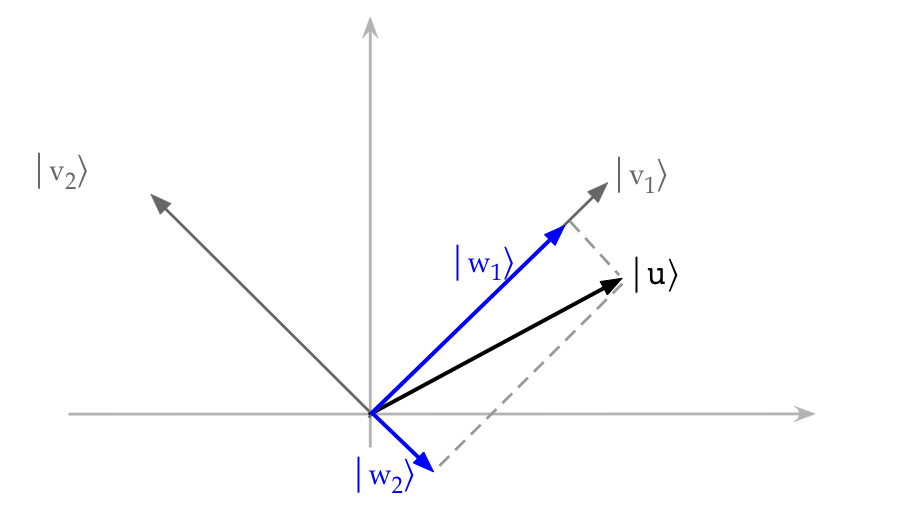
\includegraphics[width=4in]{notes/figs/n04/19basischange3.png}
        \caption{Projection}
        \label{fig:19basischange3}
    \end{figure}
    
    Here, the (real) vectors are abstract "arrows". We "numerify" an arrow when an arrow is written in terms of basis vectors. For example:
    
    $$
    |u\rangle=\frac{\sqrt{3}}{2}\left[\begin{array}{l}
    1 \\
    0
    \end{array}\right]+\frac{1}{2}\left[\begin{array}{l}
    0 \\
    1
    \end{array}\right]=\left[\begin{array}{c}
    \frac{\sqrt{3}}{2} \\
    \frac{1}{2}
    \end{array}\right]
    $$
    
    This provides coordinates in the chosen basis (the standard basis in this case). Next, observe that. The notion of projection can be described geometrically (for real vectors) without any reference to which basis vectors. More valuable, the notion of projection can be described algebraically without reference to a basis, that is, without "numerifying". For example, the projection of $|u\rangle$ along $\left|v_{1}\right\rangle$ is just $\left|v_{1}\right\rangle\left\langle v_{1}|| u\right\rangle$ whichever basis is used. What is (mathematically) interesting is that: Much of the theory can be laid out in a basis-free manner. And, in fact, can be proved for more general and abstract forms of vectors. For example: functions. One defines a vector space as a set of mathematical objects that satisfy certain rules like addition, scalar multiplication and so on. Certainly, the vectors we've seen satisfy this definition. But so do functions, which allows the theory to apply more broadly. To perform calculations (numbers!) we of course need to use some basis. The choice of basis is often up to us.

\subsection{Getting used to Dirac notation}

    Because we will see certain Dirac symbols and notation repeatedly, let's revisit parts of the previous section in this notation: First, we'll relabel the picture in Figure \ref{fig:20basischange2}.
    
    \begin{figure}
        \centering
        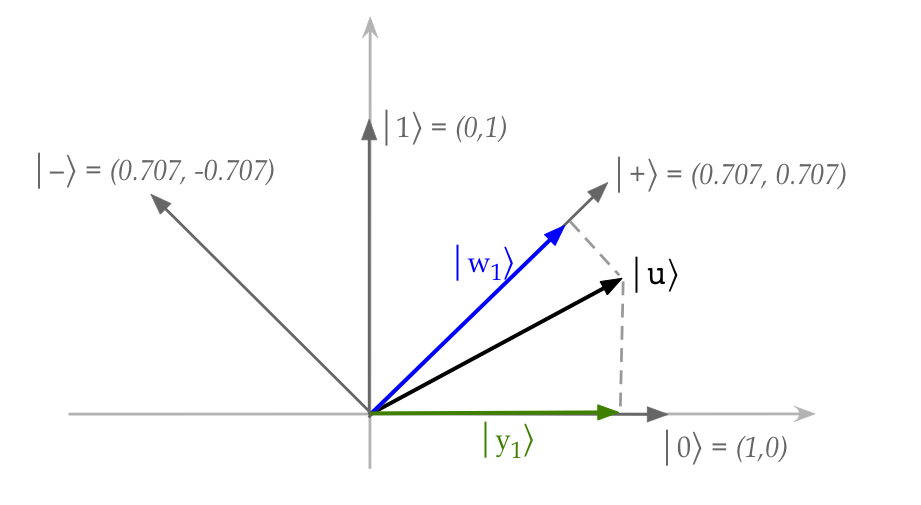
\includegraphics[width=4in]{notes/figs/n04/20basischange2.png}
        \caption{Relabeled Vector}
        \label{fig:20basischange2}
    \end{figure}
    
    Next, the standard basis vectors are written as
    
    $$
    \begin{aligned}
    &|0\rangle=\left[\begin{array}{l}
    1 \\
    0
    \end{array}\right] \\
    &|1\rangle=\left[\begin{array}{l}
    0 \\
    1
    \end{array}\right]
    \end{aligned}
    $$
    
    The second basis is called the Hadamard basis and is written as:
    
    $$
    \begin{aligned}
    &|+\rangle=\left[\begin{array}{c}
    \frac{1}{\sqrt{2}} \\
    \frac{1}{\sqrt{2}}
    \end{array}\right] \\
    &|-\rangle=\left[\begin{array}{r}
    \frac{1}{\sqrt{2}} \\
    -\frac{1}{\sqrt{2}}
    \end{array}\right]
    \end{aligned}
    $$
    
    Observe that
    
    $$
    \begin{aligned}
    &|+\rangle=\left[\begin{array}{l}
    \frac{1}{\sqrt{2}} \\
    \frac{1}{\sqrt{2}}
    \end{array}\right]=\frac{1}{\sqrt{2}}\left[\begin{array}{l}
    1 \\
    0
    \end{array}\right]+\frac{1}{\sqrt{2}}\left[\begin{array}{l}
    0 \\
    1
    \end{array}\right]=\frac{1}{\sqrt{2}}|0\rangle+\frac{1}{\sqrt{2}}|1\rangle \\
    &|-\rangle=\left[\begin{array}{r}
    \frac{1}{\sqrt{2}} \\
    -\frac{1}{\sqrt{2}}
    \end{array}\right]=\frac{1}{\sqrt{2}}\left[\begin{array}{l}
    1 \\
    0
    \end{array}\right]-\frac{1}{\sqrt{2}}\left[\begin{array}{l}
    0 \\
    1
    \end{array}\right]=\frac{1}{\sqrt{2}}|0\rangle-\frac{1}{\sqrt{2}}|1\rangle
    \end{aligned}
    $$
    
    The projector for $|0\rangle$ is:
    
    $$
    P_{0}=|0\rangle\langle 0|=\left[\begin{array}{l}
    1 \\
    0
    \end{array}\right]\left[\begin{array}{ll}
    1 & 0
    \end{array}\right]=\left[\begin{array}{ll}
    1 & 0 \\
    0 & 0
    \end{array}\right]
    $$
    
    And the projector for $|1\rangle$ is:
    
    $$
    P_{1}=|1\rangle\langle 1|=\left[\begin{array}{l}
    0 \\
    1
    \end{array}\right]\left[\begin{array}{ll}
    0 & 1
    \end{array}\right]=\left[\begin{array}{ll}
    0 & 0 \\
    0 & 1
    \end{array}\right]
    $$
    
    Similarly, the projector for $|+\rangle$ is:
    
    $$
    P_{+}=|+\rangle\langle+|=\left[\begin{array}{l}
    \frac{1}{\sqrt{2}} \\
    \frac{1}{\sqrt{2}}
    \end{array}\right]\left[\begin{array}{ll}
    \frac{1}{\sqrt{2}} & \frac{1}{\sqrt{2}}
    \end{array}\right]=\left[\begin{array}{cc}
    \frac{1}{2} & \frac{1}{2} \\
    \frac{1}{2} & \frac{1}{2}
    \end{array}\right]
    $$

\subsection{Operator-matrix and change-of-basis via sandwich and inner product}

    We'll now work through two useful results: 1. If an operator is not in matrix form, then how do we obtain its matrix? 2. How do we change coordinates from one basis to another? Although we've seen the second one before (in the Review), we'll use our newfound approach with the operator sandwich, and inner products. And at the end, we'll explain why this is a powerful tool. Let's start with the matrix of an operator: This may seem an odd objective because ... aren't all operators already matrices? In fact, no. An operator can be specified by text description. For example, let $A$ be the operator that multiplies any $2 \mathrm{D}$ vector element by 3:
    
    $$
    A|\psi\rangle=3|\psi\rangle
    $$
    
    It turns out, in this case, the matrix is:
    
    $$
    A=\left[\begin{array}{ll}
    3 & 0 \\
    0 & 3
    \end{array}\right]
    $$
    
    This is called the matrix representation of the operator $A$. What we seek: a systematic way to obtain the matrix representation. What we also seek: to directly obtain the matrix of an operator in a given basis. We'll do both with this powerful result: Suppose $\left|v_{1}\right\rangle, \ldots,\left|v_{n}\right\rangle$ is the desired basis in which we want the matrix for operator $A$. Define the numbers
    
    $$
    A_{i j} \triangleq\left\langle v_{i}|A| v_{j}\right\rangle
    $$
    
    Then the matrix for $A$ is simply the matrix with
    
    $$
    A_{i j}=\text { element in row } i, \text { column } \mathrm{j}
    $$
    
    Proposition 2.21: The matrix of an operator $A$ in an orthonormal basis $\left|v_{1}\right\rangle, \ldots,\left|v_{n}\right\rangle$ is formed by elements $A_{i j} \triangleq\left\langle v_{i}|A| v_{j}\right\rangle$ in row i and column $\mathrm{j}$. Proof: We'll do this in two steps: 1. First show that the matrix
   
    $$
    \hat{A} \triangleq \sum_{i, j} A_{i j}\left|v_{i}\right\rangle\left\langle v_{j}\right|
    $$
    
    produces the same effect as the operator $A$. 2. Then show that the i-j-th element of $\hat{A}$ is in fact $\left\langle v_{i}|A| v_{j}\right\rangle$. Let's start with the first step: First, suppose $|\phi\rangle=A|\psi\rangle$ for two vectors $|\psi\rangle$ and $|\phi\rangle$. Then, express both in the basis:
    
    $$
    \begin{aligned}
    |\psi\rangle &=\alpha_{1}\left|v_{1}\right\rangle+\ldots+\alpha_{n}\left|v_{n}\right\rangle \\
    |\phi\rangle &=\beta_{1}\left|v_{1}\right\rangle+\ldots+\beta_{n}\left|v_{n}\right\rangle
    \end{aligned}
    $$
    
    where $\alpha_{1}, \ldots, \alpha_{n}$ and $\beta_{1}, \ldots, \beta_{n}$ are the coordinates, respectively, of each of these vectors. Now, any outer-product like $\left|v_{i}\right\rangle\left\langle v_{j}\right|$ is a matrix and so
    
    $$
    \hat{A}=\sum_{i, j} A_{i j}\left|v_{i}\right\rangle\left\langle v_{j}\right|
    $$
    
    which is a linear combination of matrices is a matrix. Let's apply this matrix to $|\psi\rangle$ :
    
    $$
    \begin{aligned}
    \hat{A}|\psi\rangle &=\left(\sum_{i, j} A_{i j}\left|v_{i}\right\rangle\left\langle v_{j}\right|\right)\left(\sum_{k} \alpha_{k}\left|v_{k}\right\rangle\right.\\
    &=\sum_{i} \sum_{j} \sum_{k} \alpha_{k} A_{i j}\left|v_{i}\right\rangle\left\langle v_{j}|| v_{k}\right\rangle \\
    &=\sum_{i} \sum_{j} \sum_{k} \alpha_{k} A_{i j}\left|v_{i}\right\rangle\left\langle v_{j} \mid v_{k}\right\rangle \\
    &=\sum_{i} \sum_{j} \alpha_{j} A_{i j}\left|v_{i}\right\rangle
    \end{aligned}
    $$
    
    where the last simplification comes from the orthonormality simplification of the inner-products (the case $j=k$ and $j \neq k$ ). Next, write this last expression as
    
    $$
    \sum_{i}\left(\sum_{j} A_{i j} \alpha_{j}\right)\left|v_{i}\right\rangle
    $$
    
    Now observe: the sum inside the parentheses is the product of the i-th row of $\hat{A}$ and $|\psi\rangle$. Now compare
    
    $$
    |\phi\rangle=A|\psi\rangle
    $$
    
    with what we just derived
    
    $$
    \hat{A}|\psi\rangle=\sum_{i}\left(\sum_{j} A_{i j} \alpha_{j}\right)\left|v_{i}\right\rangle
    $$
    
    Because coefficients in a linear combination of basis vectors are unique,
    
    $$
    \beta_{i}=\left(\sum_{j} A_{i j} \alpha_{j}\right)
    $$
    
    And thus, the matrix $\hat{A}$ produces the same transformation as the operator $A$.
    Next, for step 2, let's ask: in using $\hat{A}$ for $A$, do we get the i-j-th element as $\left\langle v_{i}|A| v_{j}\right\rangle$ ? Consider $\left\langle v_{i}|A| v_{j}\right\rangle$. Substitute the matrix $\hat{A}$ :
    
    $$
    \begin{aligned}
    \left\langle v_{i}|\hat{A}| v_{j}\right\rangle &=\left\langle v_{i}\left|\sum_{m, n} A_{m, n}\right| v_{m}\right\rangle\left\langle v_{m}|| v_{j}\right\rangle \\
    &=\left\langle v_{i}\left|\sum_{m} A_{m, j}\right| v_{m}\right\rangle \\
    &=A_{i j} \\
    &=\left\langle v_{i}|A| v_{j}\right\rangle
    \end{aligned}
    $$
    
    So, the i-j-th element of $\hat{A}$ is in fact $\left\langle v_{i}|A| v_{j}\right\rangle$. Next, we'll see that a change-of-basis matrix can be written entirely with inner-products: Proposition 2.22:
    
    $$
    U_{i j}=\left\langle w_{i} \mid v_{j}\right\rangle
    $$
    
    converts coordinates from the v-basis to the w-basis. That is,
    
    $$
    \left[\begin{array}{r}
    \beta_{1} \\
    \vdots \\
    \beta_{n}
    \end{array}\right]=\left[\begin{array}{ccc}
    \left\langle w_{1} \mid v_{1}\right\rangle & \cdots & \left\langle w_{1} \mid v_{n}\right\rangle \\
    \vdots & \vdots & \vdots \\
    \left\langle w_{n} \mid v_{1}\right\rangle & \cdots & \left\langle w_{n} \mid v_{n}\right\rangle
    \end{array}\right]\left[\begin{array}{r}
    \alpha_{1} \\
    \vdots \\
    \alpha_{n}
    \end{array}\right]
    $$
    
    Proof: First note that the coordinates (coefficients) can be written as:
    
    $$
    \begin{aligned}
    \alpha_{i} &=\left\langle v_{i} \mid \psi\right\rangle \\
    \beta_{i} &=\left\langle w_{i} \mid \psi\right\rangle
    \end{aligned}
    $$
    
    Next, in the matrix-vector product above, consider the k-th row times the vector $|\psi\rangle$ : 
    
    $$
    \begin{aligned}
    &\left\langle w_{k} \mid v_{1}\right\rangle \alpha_{1}+\ldots+\left\langle w_{k} \mid v_{n}\right\rangle \alpha_{n}\\
    &=\left\langle w_{k} \mid v_{1}\right\rangle\left\langle v_{1} \mid \psi\right\rangle+\ldots+\left\langle w_{k} \mid v_{n}\right\rangle\left\langle v_{n} \mid \psi\right\rangle \quad \text { Sub for } \alpha_{i}\\
    &=\left\langle w_{k}\left|\sum_{i}\right| v_{1}\right\rangle\left\langle v_{1}|| \psi\right\rangle\\
    &=\left\langle w_{k}|I| \psi\right\rangle\\
    &=\beta_{k}
    \end{aligned}
    $$
    
    Which is indeed the k-th coordinate in the w-basis. Whew! Both were detailed multi-step proofs that required careful attention to sums. Why is this approach useful? First, it's practically useful in calculations, as we'll see below. Second, it's useful when we only have operator descriptions (as opposed to matrices). Let's apply what we've learned above: Example 1: Consider the operator that multiplies any $2 \mathrm{D}$ vector element by $3:$
    
    $$
    A|\psi\rangle=3|\psi\rangle
    $$
    
    The first thing to observe is that any matrix that multiplies basis vectors by 3 will also multiply any vector by three. This means, if we use the approach for deriving the matrix with basis vectors, it'll apply to all vectors (as desired). Let's derive the matrix using $A_{i j}=\left\langle v_{i}|A| v_{j}\right\rangle$ using the standard basis $|0\rangle,|1\rangle$ :
    
    $$
    \left[\begin{array}{ll}
    \langle 0|A| 0\rangle & \langle 0|A| 1\rangle \\
    \langle 1|A| 0\rangle & \langle 1|A| 1\rangle
    \end{array}\right]=\left[\begin{array}{ll}
    3\langle 0 \mid 0\rangle & 3\langle 0 \mid 1\rangle \\
    3\langle 0 \mid 1\rangle & 3\langle 1 \mid 1\rangle
    \end{array}\right]=\left[\begin{array}{ll}
    3 & 0 \\
    0 & 3
    \end{array}\right]
    $$
    
    Consider how we obtained the first element (top left), $\langle 0|A| 0\rangle$: First, apply $A$ to its right: $A|0\rangle=3|0\rangle$. (We know this from the description of $A$.) This results in $\langle 0|A| 0\rangle=\langle 0|3| 0\rangle=3\langle 0 \mid 0\rangle$. Now check that it works for all vectors $|\psi\rangle=\alpha|0\rangle+\beta|1\rangle$ :
    
    $$
    A|\psi\rangle=\left[\begin{array}{ll}
    3 & 0 \\
    0 & 3
    \end{array}\right]\left[\begin{array}{l}
    \alpha \\
    \beta
    \end{array}\right]=\left[\begin{array}{l}
    3 \alpha \\
    3 \beta
    \end{array}\right]=3|\psi\rangle
    $$
    
    Which it does.
    
    Example 2: Let's write the coordinate conversion matrix going from the standard to the Hadamard basis: Recall the Hadamard basis:
    
    $$
    \begin{aligned}
    |+\rangle &=\frac{1}{\sqrt{2}}|0\rangle+\frac{1}{\sqrt{2}}|1\rangle \\
    |-\rangle &=\frac{1}{\sqrt{2}}|0\rangle-\frac{1}{\sqrt{2}}|1\rangle
    \end{aligned}
    $$
    
    Note that, from this, we get
    
    $$
    \begin{aligned}
    &\langle+|=\frac{1}{\sqrt{2}}\langle 0|+\frac{1}{\sqrt{2}}\langle 1| \\
    &\langle-|=\frac{1}{\sqrt{2}}\langle 0|-\frac{1}{\sqrt{2}}\langle 1|
    \end{aligned}
    $$
    
    Next, the four inner products that will result in elements of the conversion matrix:
    
    $$
    \begin{aligned}
    &\langle+\mid 0\rangle=\left\langle\frac{1}{\sqrt{2}}\langle 0|+\frac{1}{\sqrt{2}}\langle 1|| 0\rangle=\frac{1}{\sqrt{2}}\langle 0 \mid 0\rangle+\frac{1}{\sqrt{2}}\langle 1 \mid 0\rangle=\frac{1}{\sqrt{2}}\right. \\
    &\langle+\mid 1\rangle=\left\langle\frac{1}{\sqrt{2}}\langle 0|+\frac{1}{\sqrt{2}}\langle 1|| 1\rangle=\frac{1}{\sqrt{2}}\langle 0 \mid 1\rangle+\frac{1}{\sqrt{2}}\langle 1 \mid 1\rangle=\frac{1}{\sqrt{2}}\right. \\
    &\langle-\mid 0\rangle=\left\langle\frac{1}{\sqrt{2}}\langle 0|-\frac{1}{\sqrt{2}}\langle 1|| 0\rangle=\frac{1}{\sqrt{2}}\langle 0 \mid 0\rangle-\frac{1}{\sqrt{2}}\langle 1 \mid 0\rangle=\frac{1}{\sqrt{2}}\right. \\
    &\langle-\mid 1\rangle=\left\langle\frac{1}{\sqrt{2}}\langle 0|-\frac{1}{\sqrt{2}}\langle 1|| 1\rangle=\frac{1}{\sqrt{2}}\langle 0 \mid 1\rangle-\frac{1}{\sqrt{2}}\langle 1 \mid 1\rangle=-\frac{1}{\sqrt{2}}\right.
    \end{aligned}
    $$
    
    Thus, the change-of-basis matrix is:
    
    $$
    U=\left[\begin{array}{ll}
    \langle+\mid 0\rangle & \langle+\mid 1\rangle \\
    \langle-\mid 0\rangle & \langle-\mid 1\rangle
    \end{array}\right]=\left[\begin{array}{cc}
    \frac{1}{\sqrt{2}} & \frac{1}{\sqrt{2}} \\
    \frac{1}{\sqrt{2}} & -\frac{1}{\sqrt{2}}
    \end{array}\right]
    $$
    
    Which matches what we saw earlier.
    
    Finally, let's reiterate the change-of-basis matrix for matrices: We saw this in the Review. Let's now write the same result in our new notation. Let $\left|v_{1}\right\rangle, \ldots,\left|v_{n}\right\rangle$ (v-basis) and $\left|w_{1}\right\rangle, \ldots,\left|w_{n}\right\rangle$ (w-basis) be two bases and suppose that we have an operator matrix $A_{v}$ written in the v-basis. We want the same operator matrix in the w-basis, i.e., $A_{w}$. Let $U_{v \rightarrow w}$ be the change-of-basis that converts v-basis vectors to w-basis vectors. And $U_{w \rightarrow v}$ be the change-of-basis that converts w-basis vectors to v-basis vectors. Then
    
    $$
    A_{w}=U_{v \rightarrow w} A_{v} U_{w \rightarrow v}
    $$
    
    To highlight this, we'll write this up as a proposition. Proposition 2.23:
    
    $$
    A_{w}=U_{v \rightarrow w} A_{v} U_{w \rightarrow v}
    $$
    
    where $U_{v \rightarrow w}$ and $U_{w \rightarrow v}$ are the change-of-basis matrices going from one to the other basis. Proof: See earlier Review. Let's apply this in an example: Suppose we are in the $|+\rangle,|-\rangle$ basis (H-basis) and we have the operator
    
    $$
    X=\left[\begin{array}{ll}
    0 & 1 \\
    1 & 0
    \end{array}\right]
    $$
    
    in the same basis. As an example of applying it:
    
    $$
    x|+\rangle=\left[\begin{array}{ll}
    0 & 1 \\
    1 & 0
    \end{array}\right]\left[\begin{array}{l}
    1 \\
    0
    \end{array}\right]=\left[\begin{array}{l}
    0 \\
    1
    \end{array}\right]=|-\rangle
    $$
    
    We'd like to have the operator in standard coordinates. We've already derived the conversion matrix from standard to H-basis:
    
    $$
    U_{S \rightarrow H}=\left[\begin{array}{cc}
    \frac{1}{\sqrt{2}} & \frac{1}{\sqrt{2}} \\
    \frac{1}{\sqrt{2}} & -\frac{1}{\sqrt{2}}
    \end{array}\right]
    $$
    
    It's easy to show that the inverse, $U_{H \rightarrow S}$, is the same: $U_{S \rightarrow H}$. From this, we can convert $X$ to the standard basis. Let's call the result $X_{S}$
    
    $$
    X_{S}=U_{S \rightarrow H} X U_{H \rightarrow S}=\left[\begin{array}{cc}
    \frac{1}{\sqrt{2}} & \frac{1}{\sqrt{2}} \\
    \frac{1}{\sqrt{2}} & -\frac{1}{\sqrt{2}}
    \end{array}\right]\left[\begin{array}{ll}
    0 & 1 \\
    1 & 0
    \end{array}\right]\left[\begin{array}{cc}
    \frac{1}{\sqrt{2}} & \frac{1}{\sqrt{2}} \\
    \frac{1}{\sqrt{2}} & -\frac{1}{\sqrt{2}}
    \end{array}\right]=\left[\begin{array}{cc}
    1 & 0 \\
    0 & -1
    \end{array}\right]
    $$
    
    Then, applying it in the standard basis, we get the same result as before $X|+\rangle=|-\rangle$ but now in standard coordinates:
    
    $$
    X_{S}|+\rangle=\left[\begin{array}{cc}
    1 & 0 \\
    0 & -1
    \end{array}\right]\left[\begin{array}{c}
    \frac{1}{\sqrt{2}} \\
    \frac{1}{\sqrt{2}}
    \end{array}\right]=\left[\begin{array}{c}
    \frac{1}{\sqrt{2}} \\
    -\frac{1}{\sqrt{2}}
    \end{array}\right]=|-\rangle
    $$

\subsection{Orthogonal subspaces}

    Let's return to the idea of a vector space: Suppose $\left|v_{1}\right\rangle, \ldots,\left|v_{n}\right\rangle$ is a basis for $\mathrm{n}$-component complex vectors. The set
    
    $$
    \begin{aligned}
    V &=\operatorname{span}\left\{\left|v_{1}\right\rangle,\left|v_{2}\right\rangle, \ldots,\left|v_{n}\right\rangle\right\} \\
    &=\left\{\alpha_{1}\left|v_{1}\right\rangle+\alpha_{2}\left|v_{2}\right\rangle+\ldots+\alpha_{k}\left|v_{n}\right\rangle: \alpha_{i} \in \mathbb{C}\right\}
    \end{aligned}
    $$
    
    is a vector space, meaning that all linear combinations of any subset of vectors in $V$ is in $V$. Another way of saying this: $V$ is closed under linear combinations. Now consider just the span of the first two of these vectors:
    
    $$
    \begin{aligned}
    W &=\operatorname{span}\left\{\left|v_{1}\right\rangle,\left|v_{2}\right\rangle\right\} \\
    &=\left\{\alpha_{1}\left|v_{1}\right\rangle+\alpha_{2}\left|v_{2}\right\rangle: \alpha_{i} \in \mathbb{C}\right\}
    \end{aligned}
    $$
    
    Is this a vector space? Let's test: Let's, for example, pick three vectors in $W$ and ask if the linear combination is in $W$ :

    $$
    \begin{aligned}
    \left|x_{1}\right\rangle &=a_{1}\left|v_{1}\right\rangle+a_{2}\left|v_{2}\right\rangle \\
    \left|x_{2}\right\rangle &=b_{1}\left|v_{1}\right\rangle+b_{2}\left|v_{2}\right\rangle \\
    \left|x_{3}\right\rangle &=c_{1}\left|v_{1}\right\rangle+c_{2}\left|v_{2}\right\rangle
    \end{aligned}
    $$
    
    A linear combination of these three is:
    
    $$
    |z\rangle=\beta_{1}\left|x_{1}\right\rangle+\beta_{2}\left|x_{2}\right\rangle+\beta_{3}\left|x_{3}\right\rangle
    $$
    
    We want to ask: is $|z\rangle \in W$ ? The exercise below shows that it does. Observe: Every vector in $W$ is in $V$. Not every vector in $V$ is in $W$. Thus, we say $W$ is a subspace of $V$. Now consider the set $W^{\prime}$ :
    
    $$
    W^{\prime}=\operatorname{span}\left\{\left|v_{3}\right\rangle, \ldots,\left|v_{n}\right\rangle\right\}
    $$
    
    One can see that $W^{\prime}$ is also a subspace of $V$. Now, there's a complementary relationship between $W$ and $W^{\prime}$ : Suppose $|x\rangle \in W$ and $|y\rangle \in W^{\prime}$. Then we can use the basis vectors to express them: $|x\rangle=a_{1}\left|v_{1}\right\rangle+a_{2}\left|v_{2}\right\rangle$,  $|y\rangle=a_{3}\left|v_{3}\right\rangle+\ldots+a_{n}\left|v_{n}\right\rangle$ Then
    
    $$
    \begin{aligned}
    \langle x \mid y\rangle &=\left\langle a_{1}^{*}\left\langle v_{1}\left|+a_{2}^{*}\left\langle v_{2}|| a_{3} \mid v_{3}\right\rangle+\ldots+a_{n}\right| v_{n}\right\rangle\right\rangle \\
    &=0
    \end{aligned}
    $$
    
    because the $\left|v_{i}\right\rangle$ 's are orthogonal. Thus, every vector in $W$ is orthogonal to every vector in $W^{\prime}$. Two subspaces that satisfy this property are said to be orthogonal complements: We use the notation $W^{\perp}=$ orthogonal complement subspace to $W$. Here, $W^{\perp}=W^{\prime}$ Notice also that 
    
    $$
    W \cup W^{\prime}=V
    $$
    
    That is, if we pull into one set every vector in each of $W, W^{\prime}$ we'll get all the vectors in $V$. This notion can extend to multiple subspaces: For example, suppose $W_{3}=\operatorname{span}\left\{\left|v_{3}\right\rangle\right\}, W_{4}=\operatorname{span}\left\{\left|v_{4}\right\rangle\right\}, \ldots, W_{n}=\operatorname{span}\left\{\left|v_{n}\right\rangle\right\}$ Then any two of these are orthogonal, and all of them are orthogonal to $W=\operatorname{span}\left\{\left|v_{1}\right\rangle,\left|v_{2}\right\rangle\right\}$. And
    
    $$
    W \cup W_{3} \cup \ldots \cup W_{n}=V
    $$

    Projectors for subspaces: Recall the definitions of $V$ and $W$ from above:
    
    $$
    \begin{aligned}
    V &=\operatorname{span}\left\{\left|v_{1}\right\rangle,\left|v_{2}\right\rangle, \ldots,\left|v_{n}\right\rangle\right\} \\
    W &=\operatorname{span}\left\{\left|v_{1}\right\rangle,\left|v_{2}\right\rangle\right\}
    \end{aligned}
    $$
    
    Let's pick a generic vector in $V$ from above:
    
    $$
    |u\rangle=a_{1}\left|v_{1}\right\rangle+a_{2}\left|v_{2}\right\rangle+\ldots+a_{n}\left|v_{n}\right\rangle
    $$
    
    Define the matrix
    
    $$
    \begin{aligned}
    P_{v_{1}, v_{2}} &=P_{v_{1}}+P_{v_{2}} & & \text { Projectors for each of }\left|v_{1}\right\rangle,\left|v_{2}\right\rangle \\
    &=\left|v_{1}\right\rangle\left\langle v_{1}|+| v_{2}\right\rangle\left\langle v_{2}\right| & & \text { Each projector is an outer-product }
    \end{aligned}
    $$
    
    Let's apply this to the vector $|u\rangle$ :
    
    $$
    \begin{aligned}
    P_{v_{1}, v_{2}}|u\rangle=&\left(\left|v_{1}\right\rangle\left\langle v_{1}|+| v_{2}\right\rangle\left\langle v_{2}\right|\right)\left(a_{1}\left|v_{1}\right\rangle+a_{2}\left|v_{2}\right\rangle+\ldots+a_{n}\left|v_{n}\right\rangle\right) \\
    =&\left(a_{1}\left|v_{1}\right\rangle\left\langle\mathbf{v}_{\mathbf{1}} \mid \mathbf{v}_{\mathbf{1}}\right\rangle+a_{2}\left|v_{1}\right\rangle\left\langle v_{1} \mid v_{2}\right\rangle+\ldots+a_{n}\left|v_{1}\right\rangle\left\langle v_{1} \mid v_{n}\right\rangle\right) \\
    &+\left(a_{1}\left|v_{1}\right\rangle\left\langle v_{2} \mid v_{1}\right\rangle+a_{2}\left|v_{1}\right\rangle\left\langle\mathbf{v}_{\mathbf{2}} \mid \mathbf{v}_{2}\right\rangle+\ldots+a_{n}\left|v_{1}\right\rangle\left\langle v_{2} \mid v_{n}\right\rangle\right) \\
    =& a_{1}\left|v_{1}\right\rangle+a_{2}\left|v_{2}\right\rangle
    \end{aligned}
    $$
    
    (Only the two bolded inner products are non-zero.) The result is a vector in $W$. This is called the projection of $|u\rangle$ onto the subspace $W$. In this way, if $S \subset V$ is any subspace of $V$, with basis $\left|s_{1}\right\rangle,\left|s_{2}\right\rangle, \ldots,\left|s_{k}\right\rangle$, then the projector for this subspace is:
    
    $$
    P_{S}=\left|s_{1}\right\rangle\left\langle s_{2}|+\ldots+| s_{k}\right\rangle\left\langle s_{k}\right|
    $$
    
    This means that if $|u\rangle \in V$ is any vector in $V$, the vector $P_{S}|u\rangle \in S$. Important: the projected vectors are not necessarily unit-length. Example: Suppose $V=\operatorname{span}\{|0\rangle,|1\rangle\}$. Let $S=\operatorname{span}\{|0\rangle\}$ be a subspace. Then the projector is $P_{S}=|0\rangle\langle 0|$. Let
    
    $$
    |u\rangle=\frac{1}{\sqrt{2}}|0\rangle+\frac{1}{\sqrt{2}}|1\rangle
    $$
    
    be a vector in $V$. Then

    $$
    \begin{aligned}
    P_{S}|u\rangle &=|0\rangle\left\langle0 \left|\left(\frac{1}{\sqrt{2}}|0\rangle+\frac{1}{\sqrt{2}}|1\rangle\right)\right.\right.\\
    &=\frac{1}{\sqrt{2}}|0\rangle\langle 0 \mid 0\rangle+\frac{1}{\sqrt{2}}|0\rangle\langle 0 \mid 1\rangle \\
    &=\frac{1}{\sqrt{2}}|0\rangle
    \end{aligned} 
    $$

    (Recall: $|0\rangle\langle 1|=0$ ). Then the length of this result is:
    
    $$
    \left.\left|P_{S}\right| u\right\rangle|=| \frac{1}{\sqrt{2}}|0\rangle \mid=\frac{1}{\sqrt{2}}
    $$
    
    Why are projectors important? Projectors are how the critical action of measurement occurs in quantum computing (and mechanics). A stronger understanding of this part of the theory makes it less mysterious than it first appears to be. Next, let's work through an example: Recall
    
    $$
    |+\rangle=\frac{1}{\sqrt{2}}|0\rangle+\frac{1}{\sqrt{2}}|1\rangle
    $$
    
    Let's apply the projector for $\operatorname{span}\{|+\rangle\}$ to the vector $|0\rangle$. First, the projector:
    
    $$
    P_{+}=\left[\begin{array}{c}
    \frac{1}{\sqrt{2}} \\
    \frac{1}{\sqrt{2}}
    \end{array}\right]\left[\begin{array}{ll}
    \frac{1}{\sqrt{2}} & \frac{1}{\sqrt{2}}
    \end{array}\right]=\left[\begin{array}{cc}
    \frac{1}{2} & \frac{1}{2} \\
    \frac{1}{2} & \frac{1}{2}
    \end{array}\right]
    $$
    
    Now apply to $|0\rangle$ :
    
    $$
    P_{+}|0\rangle=\left[\begin{array}{ll}
    \frac{1}{2} & \frac{1}{2} \\
    \frac{1}{2} & \frac{1}{2}
    \end{array}\right]\left[\begin{array}{l}
    1 \\
    0
    \end{array}\right]=\left[\begin{array}{c}
    \frac{1}{2} \\
    \frac{1}{2}
    \end{array}\right]=\frac{1}{\sqrt{2}}|+\rangle
    $$

    The special case of 2D: Consider the 2D vector $|0\rangle$. Let's ask: which unit-length 2D vectors $\left|w^{\perp}\right\rangle$ are orthogonal to $|w\rangle=|0\rangle$ ? Write
    
    $$
    \left|w^{\perp}\right\rangle=\alpha|0\rangle+\beta|1\rangle
    $$
    
    in terms of the standard basis. For orthogonality,
    
    $$
    \begin{aligned}
    &\left\langle 0 \mid w^{\perp}\right\rangle=0 \\
    &\langle 0|\alpha| 0\rangle+\beta|1\rangle\rangle=0 \\
    &\langle 0|\alpha| 0\rangle+\beta|1\rangle\rangle=0 \\
    &\alpha=0 \\
    &\left|w^{\perp}\right\rangle=\beta|1\rangle
    \end{aligned}
    $$
    
    For unit-length, we must have
    
    $$
    \begin{array}{lcl} 
    & \left\langle w^{\perp} \mid w^{\perp}\right\rangle & =1 \\
    \Rightarrow & \left\langle\beta^{*}\langle 1|| \beta \mid 1\rangle\right\rangle & =1 \\
    \Rightarrow & \beta^{*} \beta\langle 1 \mid 1\rangle & =1 \\
    \Rightarrow & |\beta|=1 &
    \end{array}
    $$
    
    Thus, $\beta$ can be any complex number of unit magnitude. Example: $\beta=1$
    
    $$
    \triangleright\left|w^{\perp}\right\rangle=|1\rangle
    $$
    
    Notice that all the vectors orthogonal to $|w\rangle=|0\rangle$ are along $\left|w^{\perp}\right\rangle=|1\rangle$. In some sense, there's only one vector along which lie the orthogonal vectors to $|w\rangle=|0\rangle$. This is not true for 3D and higher: For example, with real vectors, consider $|w\rangle=(1,0,0)$ in 3D. Any vector in the $y$-z plane is perpendicular (orthogonal) to $|w\rangle$. And there are an infinite number of them in an infinite number of directions. When working with single qubits, this observation will be useful, so let's generalize and observe the following: Suppose $|v\rangle$ and $\left|v^{\perp}\right\rangle$ are two basis vectors for 2D. Let $|w\rangle=a|v\rangle+b\left|v^{\perp}\right\rangle$ Then $\left|w^{\perp}\right\rangle=b^{*}|v\rangle-a^{*}\left|v^{\perp}\right\rangle$ is orthogonal because
    
    $$
    \begin{aligned}
    \left\langle w \mid w^{\perp}\right\rangle &=\left\langle a^{*}\left\langle v\left|+b^{*}\left\langle v^{\perp}|| b^{*} \mid v\right\rangle-a^{*}\right| v^{\perp}\right\rangle\right\rangle \\
    &=a^{*} b^{*}\langle v \mid v\rangle-b^{*} a^{*}\left\langle v^{\perp} \mid v^{\perp}\right\rangle \\
    &=0
    \end{aligned}
    $$

\subsection{A mathematical aside}

    For the theoretically inclined, we'll point out a few things, none of which are essential to the course but which might stimulate further curiosity: All the theory laid out in this module was done so with complex vectors and matrices. The advantage of abstraction is wider applicability, and the satisfaction of seeing the common features work for both quantum computing and mechanics. The advantage of the vector approach, instead, is that it's generally easier to work with and understand. What we recommend: start from the concrete to develop skill and concepts, and then move on to the abstract as necessary. Some theoretical results of interest: There is a broader category of operator called normal: $A$ is normal if $A A^{\dagger}=A^{\dagger} A$ : Any Hermitian or unitary operator is also normal. Normal operators have an orthonormal basis of eigenvectors. Many results have an if-and-only-if character, for example: If an operator $A$ satisfies any of the properties of unitary operators described above, it must be unitary. Any operator whose eigenvectors form a basis must be normal.

\subsection{Summary}

    This was one long module, packed with new concepts and notation all at once. Understandably, this will take time to digest and make your own. The most reliable way is: repetition. The third time you return to something and read/write/solve, you will be a lot more at ease. The notion that one can compute using the elements of complex linear algebra seems alien at this time: After all, with regular linear algebra, vectors and matrices are things you "do math with". Writing code for matrices/vectors involves the usual loops, conditionals, arrays. But in quantum computing, there are no such things as loops, conditionals and arrays. Instead, one writes "programs" with vectors and unitary matrices, with the occasional use of projectors. At this time, you might be curious about: What exactly do complex vectors represent? Why did we use such gnarly numbers like $\frac{1}{\sqrt{2}}$ ? How do complex vectors feature in algorithms that, for example, factor integers (Shor's algorithm that breaks conventional crypto). Why are complex vectors the fundamental building blocks? Couldn't a simpler non-complex theory work? We'll answer these in due time. The best thing to do right now is to re-read this module so as to get more comfortable with Dirac notation.

\end{document}